% Se puede agregar el argumento 'twoside' a la par de letterpaper si se
% quiere imprimir dúplex, como libro
\documentclass[10pt, letterpaper]{report}
\usepackage[spanish,mexico]{babel}
\selectlanguage{spanish}
\usepackage[utf8]{inputenc}
\usepackage[T1]{fontenc}

\title{Plantilla para Trabajos de Graduación UVG}
\author{MSc. Miguel Zea}
\date{\today}

% Comandos definidos por el usuario en el archivo comandos_usuario.tex
%% Denominaciones coherentes con la Guía UVG y con las referencias del texto.
% Se aplicaron después de cargar babel y al iniciar el documento.
\addto\captionsspanish{%
    \renewcommand{\tablename}{Cuadro}%
    \renewcommand{\listtablename}{Lista de cuadros}%
    \renewcommand{\listfigurename}{Lista de figuras}%
}
\AtBeginDocument{%
    \renewcommand{\tablename}{Cuadro}%
    \renewcommand{\listtablename}{Lista de cuadros}%
    \renewcommand{\listfigurename}{Lista de figuras}%
}


% Información del estudiante en el archivo datos_estudiante.tex
% ================================================================================
% El estudiante debe llenar sus datos en esta sección para que la plantilla los 
% auto-importe y genere automáticamente las páginas de portada y de firmas 
% autorizadas.
% ================================================================================
% Datos del estudiante:
% --------------------------------------------------------------------------------
% Nombre completo
\def \nombreestudiante {Edgar Samuel Chavarría Castañón}
% Carné
\def \uvgcarne {22055}
% Facultad
\def \uvgfacultad {Ingeniería}
% Carrera
\def \uvgcarrera {Ingeniería Mecatronica}

% Datos del trabajo:
% --------------------------------------------------------------------------------
% Título completo
\def \titulotesis {Reingeniería mecánica y automatización de un brazo robótico cartesiano mediante la integración de sistemas de visión computacional y sensores para el proceso de manipulación y transferencia de productos en la línea de empaque del Laboratorio de Diseño de Procesos de la UVG.}
% Mes de entrega
\def \mesentrega {octubre }
% Año de entrega
\def \anoentrega {2026}
% Asesor
\def \nombreasesor {Inga. Dulce María Chacón Muñoz}

% Datos del tribunal examinador:
% --------------------------------------------------------------------------------
% Nombre del primer examinador
\def \nombreprimerex {MSc. Carlos Juárez}
% Nombre del segundo examinador
\def \nombresegundoex {Ing. Luis Pedro Gonzáles}
% Fecha de aprobación
\def \fechaaprobacion {5 de diciembre de 2018}

% Capítulos pre-definidos
% --------------------------------------------------------------------------------
% Comentar las líneas de las secciones que desean omitirse, por defecto se 
% se incluyen todas.
\def \CAPprefacio {Prefacio}
\def \CAPagradecimientos {Agradecimientos}
\def \CAPantecedentes {Antecedentes}
\def \CAPalcance {Alcance}
\def \CAPanexos {Anexos}
\def \CAPglosario {Glosario}
\def \CAPsimbolos {Listado de símbolos}

% Formato y estilo de la plantilla
% --------------------------------------------------------------------------------
% Portada: Puede cambiarse la imagen en la portada al cambiar el nombre del 
% archivo siguiente. NOTA: debe tener la suficiente resolución para cubrir el área
% designada
\def \imagenportada {plantilla/portadacit.jpg}
% Referencias: Puede des-comentar la siguiente línea para utilizar el formato de referencias APA
%\def \usarAPA {Usar formato APA}
% Párrafo: Puede comentar la siguiente línea si desea emplear un formato de 
% párrafo distinto al establecido por defecto
\def \parpordefecto {Formato de párrafo por defecto}
% Capítulos y secciones: Puede des-comentar la siguiente línea para establecer el 
% formato de los capítulos y secciones bajo el estándar original de UVG para
% trabajos de graduación. Este incluye: capítulos con numeración romana, secciones
% con letras mayúsculas, sub-secciones con números y sub-sub-secciones con letras
% minúsculas
%\def \capsecuvg {Formato UVG para capítulos y secciones}
% ================================================================================
% En este archivo se colocan opciones adicionales para modificar el formato de la
% plantilla, para emplearse en otros tipos de documentos que no sean trabajos de
% graduación. Si usted está trabajando su tesis, NO modifique este archivo
% ================================================================================
% Capítulos pre-definidos
% --------------------------------------------------------------------------------
% Comentar las líneas de las secciones que desean omitirse, por defecto se 
% se incluyen todas.
\def \CAPportada {Portada}
\def \CAPcaratula {Caratula}
\def \CAPfirmas {Hoja de firmas}
\def \CAPindice {Índice general}
\def \CAPfiguras {Listado de figuras}
\def \CAPcuadros {Listado de cuadros}
\def \CAPresumen {Resumen}
\def \CAPintroduccion {Introducción}
\def \CAPobjetivos {Objetivos}
\def \CAPjustificacion {Justificación}
\def \CAPmarcoteorico {Marco teórico}
\def\CAPresultados{Resultados}
\def\CAPdicusion{Discusión}
\def \CAPconclusiones {Conclusiones}
\def \CAPrecomendaciones {Recomendaciones}
\def \CAPbibliografia {Bibliografía}

% ================================================================================
% DEFINICIÓN DE PAQUETES
% ================================================================================
\usepackage{xcolor}
\usepackage{amsfonts}
\usepackage{amsmath}
\usepackage{amssymb}
\usepackage{amsthm}
\usepackage{amsfonts}
\usepackage{mathtools}
\usepackage{graphicx}
\usepackage{xfrac}
\usepackage{float}
\usepackage{mathtools}
\usepackage[hypertexnames=false]{hyperref}
% \usepackage{bookmark}
\usepackage{subcaption}
\usepackage{babelbib}
\ifdefined\usarAPA 
	\usepackage{apacite} 
\fi
\usepackage[percent]{overpic}

\ifdefined\CAPglosario
	\usepackage[toc]{glossaries}
	\makeglossaries
    \newglossaryentry{latex}
{
    name=latex,
    description={Es un lenguaje de marcado adecuado especialmente para la creación de documentos científicos}
} 
 
\newglossaryentry{formula}
{
    name=fórmula,
    description={Una expresión matemática} 
}
\fi
\ifdefined\CAPsimbolos
	\usepackage[intoc, spanish]{nomencl}
	\makenomenclature
    \nomenclature{$c$}{Velocidad de la luz en el vacío}
\nomenclature{$h$}{Constante de Plank}
    \renewcommand{\nomname}{Lista de Símbolos}
\fi

% ================================================================================
% MÁRGENES Y FORMATO GENERALES
% ================================================================================
\usepackage[top=1in, left=1.5in, right=1in, bottom=1in]{geometry}
%Options: Sonny, Lenny, Glenn, Conny, Rejne, Bjarne, Bjornstrup
\usepackage[Sonny]{fncychap}
% ================================================================================
% DEFINICIONES DE LA PLANTILLA
% ================================================================================
\definecolor{uvg-green}{RGB}{17,71,52}
\newcommand{\defaultparformat}[1]{
	{\setlength{\parskip}{2ex}
    \input{#1}}
}
\ifdefined\capsecuvg
	\renewcommand\thechapter{\Roman{chapter}}
    \renewcommand\thesection{\Alph{section}}
	\renewcommand\thesubsection{\arabic{subsection}}
    \renewcommand\thesubsubsection{\alph{subsubection}}
\fi
% ================================================================================

% Comandos definidos por el usuario en el archivo comandos_usuario.tex
% Denominaciones coherentes con la Guía UVG y con las referencias del texto.
% Se aplicaron después de cargar babel y al iniciar el documento.
\addto\captionsspanish{%
    \renewcommand{\tablename}{Cuadro}%
    \renewcommand{\listtablename}{Lista de cuadros}%
    \renewcommand{\listfigurename}{Lista de figuras}%
}
\AtBeginDocument{%
    \renewcommand{\tablename}{Cuadro}%
    \renewcommand{\listtablename}{Lista de cuadros}%
    \renewcommand{\listfigurename}{Lista de figuras}%
}


% ================================================================================
% CUERPO DEL TRABAJO
% ================================================================================
\pagestyle{headings}
\begin{document}
% ================================================================================
% PORTADA
% ================================================================================
%
% ================================================================================
% PRIMERA PÁGINA
% ================================================================================

% ================================================================================
% PRIMERA PÁGINA (CARÁTULA DOBLE CON PÁGINA EN BLANCO)
% ================================================================================
\ifdefined\CAPcaratula
    \newpage
    \pagecolor{white}
    \color{black}
    \setcounter{page}{1}
    \pagenumbering{roman}
    
    % --- PRIMERA CARÁTULA ---
    \thispagestyle{empty}
    \begin{center}
        \LARGE UNIVERSIDAD DEL VALLE DE GUATEMALA\\
        \LARGE Facultad de \uvgfacultad \\[0.75cm]
    \end{center}
    \begin{figure}[h]
        \begin{center}
        
\includegraphics[height=5.5 cm]{plantilla/escudoUVGnegro.eps}
        \vspace{0.5in}
        \end{center}
    \end{figure}
    \begin{center}
        \LARGE \textbf{\titulotesis} \\
        \vfill
        \vfill
        \Large Trabajo de graduación en modalidad de Trabajo Profesional presentado por Edgar Samuel Chavarría Castañón para optar al grado académico de Licenciado en Ingenieria Mecatronica \\
        %\Large \nombreestudiante \\
       % \Large Para optar al grado académico de Licenciado en \uvgcarrera \\
        \vfill
        \large Guatemala, \mesentrega del \anoentrega
    \end{center}

    % --- PÁGINA EN BLANCO ---
    \newpage
    \thispagestyle{empty}
    \mbox{} % Este comando es clave para que LaTeX imprima una página vacía real
    
    % --- SEGUNDA CARÁTULA ---
    \newpage
    \thispagestyle{empty}
    \begin{center}
        \LARGE UNIVERSIDAD DEL VALLE DE GUATEMALA\\
        \LARGE Facultad de \uvgfacultad \\[0.75cm]
    \end{center}
    \begin{figure}[h]
        \begin{center}
        
\includegraphics[height=5.5 cm]{plantilla/escudoUVGnegro.eps}
        \vspace{0.5in}
        \end{center}
    \end{figure}
    \begin{center}
        \LARGE \textbf{\titulotesis} \\
        \vfill
        \vfill
        \Large Trabajo de graduación en modalidad de Trabajo Profesional presentado por Edgar Samuel Chavarría Castañón para optar al grado académico de Licenciado en Ingenieria Mecatronica \\
        %\Large \nombreestudiante \\
        %\Large Para optar al grado académico de Licenciado en \uvgcarrera \\
        \vfill
        \large Guatemala, \mesentrega del \anoentrega
    \end{center}
\fi

% ================================================================================
% HOJA DE FIRMAS
% ================================================================================
\ifdefined\CAPfirmas
	\newpage
	\thispagestyle{empty}
	\vspace*{0.5in}
	\large Vo.Bo.:\\[1cm]
	\begin{center}
		(f) \rule[1pt]{4 in}{1pt}\\
		\nombreasesor
	\end{center}
	\vspace{1in}

	% Tribunal Examinador:\\[1cm]
	% \begin{center}
	% 	(f) \rule[1pt]{4 in}{1pt}\\
	% 	\nombreasesor \\[1in]
	% 	(f) \rule[1pt]{4 in}{1pt}\\
	% 	\nombreprimerex \\[1in]
	% 	(f) \rule[1pt]{4 in}{1pt}\\
	% 	\nombresegundoex
	% \end{center}
	% \vspace{1in}

	%Fecha de aprobación: Guatemala, \fechaaprobacion.
	\normalsize
\fi

% ================================================================================
% PREFACIO
% ================================================================================
% \ifdefined\CAPprefacio
% 	\newpage
% 	\cleardoublepage\phantomsection
%     \chapter*{Prefacio}
%     \ifdefined\parpordefecto
%     	\defaultparformat{prefacio}
%     \else
%     	% Lorem ipsum dolor sit amet, consectetur adipiscing elit. Cras vitae eleifend ipsum, ut mattis nunc. Pellentesque ac hendrerit lacus. Cras sollicitudin eget sem nec luctus. Vivamus aliquet lorem id elit venenatis pellentesque. Nam id orci iaculis, rutrum ipsum vel, porttitor magna. Etiam molestie vel elit sed suscipit. Proin dui risus, scelerisque porttitor cursus ac, tempor eget turpis. Aliquam ultricies congue ligula ac ornare. Duis id purus eu ex pharetra feugiat. Vivamus ac orci arcu. Nulla id diam quis erat rhoncus hendrerit. Class aptent taciti sociosqu ad litora torquent per conubia nostra, per inceptos himenaeos. Sed vulputate, metus vel efficitur fringilla, orci ex ultricies augue, sit amet rhoncus ex purus ut massa. Nam pharetra ipsum consequat est blandit, sed commodo nunc scelerisque. Maecenas ut suscipit libero. Sed vel euismod tellus.

% Proin elit tellus, finibus et metus et, vestibulum ullamcorper est. Nulla viverra nisl id libero sodales, a porttitor est congue. Maecenas semper, felis ut rhoncus cursus, leo magna convallis ligula, at vehicula neque quam at ipsum. Integer commodo mattis eros sit amet tristique. Cras eu maximus arcu. Morbi condimentum dignissim enim non hendrerit. Sed molestie erat sit amet porttitor sagittis. Maecenas porttitor tincidunt erat, ac lacinia lacus sodales faucibus. Integer nec laoreet massa. Proin a arcu lorem. Donec at tincidunt arcu, et sodales neque. Morbi rhoncus, ligula porta lobortis faucibus, magna diam aliquet felis, nec ultrices metus turpis et libero. Integer efficitur erat dolor, quis iaculis metus dignissim eu.
%     \fi
%     \addcontentsline{toc}{chapter}{Prefacio}
% \fi

% ================================================================================
% ÍNDICE GENERAL
% ================================================================================
\ifdefined\CAPindice
	\newpage
    %\cleardoublepage\phantomsection
	\renewcommand{\contentsname}{Índice}
    \phantomsection
    \pdfbookmark{\contentsname}{toc}
	\tableofcontents
\fi

% ================================================================================
% LISTADOS DE FIGURAS Y CUADROS
% ================================================================================
\ifdefined\CAPfiguras
    \clearpage
    \phantomsection
    \addcontentsline{toc}{chapter}{Lista de figuras}
    \listoffigures
\fi
\ifdefined\CAPcuadros
    \clearpage
    \phantomsection
    \addcontentsline{toc}{chapter}{Lista de cuadros}
    \listoftables
\fi


% ================================================================================
% AGRADECIMIENTOS
% ================================================================================
% \ifdefined\CAPagradecimientos
% 	\newpage
%     \cleardoublepage\phantomsection
% 	\chapter*{Agradecimientos}
% 	\ifdefined\parpordefecto
%     	\defaultparformat{agradecimientos}
%     \else
%     	\input{agradecimientos}
%     \fi 
% 	\addcontentsline{toc}{chapter}{Agradecimientos}
% \fi





% ================================================================================
% RESUMEN
% ================================================================================
\ifdefined\CAPresumen
	\newpage
    \cleardoublepage\phantomsection
	\chapter*{Resumen}
	\ifdefined\parpordefecto
		\defaultparformat{resumen}
	\else
		El presente trabajo abordó la reingeniería mecánica y la automatización de un brazo robótico cartesiano existente para su aplicación en la línea de empaque del Laboratorio de Diseño de Procesos de la Universidad del Valle de Guatemala. El sistema existente presentaba limitaciones mecánicas en los ejes X, Y y Z, entre ellas fricción elevada, desalineaciones y movimientos irregulares, las cuales afectaban su precisión, repetibilidad y capacidad de operar de forma estable. Para corregir estas deficiencias, se rediseñaron parcialmente los componentes estructurales y los sistemas de traslación mediante herramientas de diseño asistido por computadora. Asimismo, se incorporaron ejes guía y rodamientos lineales con el propósito de mejorar la fluidez y estabilidad del movimiento.

La automatización del sistema se desarrolló mediante una arquitectura de control embebido encargada de coordinar los motores, sensores, dispositivos de comunicación y periféricos. Se integraron finales de carrera para realizar la calibración automática y establecer referencias de movimiento, así como un codificador rotativo para medir la velocidad de la banda transportadora y facilitar la sincronización del proceso. Además, se implementó un sistema de visión computacional para identificar objetos con características previamente definidas, como figura y color, y determinar la información necesaria para ejecutar tareas de detección, clasificación, manipulación y transferencia mediante una secuencia de tipo \textit{pick and place}. El brazo también contó con un modo de operación manual mediante un mando inalámbrico y una interfaz local para visualizar el estado de calibración, el modo de operación y las acciones realizadas por el sistema.

La metodología se organizó en fases de evaluación del mecanismo existente, rediseño mecánico, fabricación y ensamblaje, desarrollo de la arquitectura electrónica, programación del control de movimiento, integración del sistema de visión y validación experimental. Las pruebas se realizaron en un entorno académico controlado y permitieron evaluar variables como la precisión de posicionamiento, la repetibilidad, el tiempo de respuesta, la capacidad de detección de objetos y el funcionamiento general del sistema. Para ello, se ejecutaron movimientos y ciclos repetitivos, se compararon las posiciones alcanzadas con las posiciones objetivo y se analizó la variación entre distintas ejecuciones.

Como resultado, se obtuvo un brazo robótico cartesiano con un movimiento más fluido, estable y repetible, capaz de ejecutar tareas automatizadas de manipulación y transferencia de productos dentro de una línea de empaque simulada. Asimismo, el sistema se desarrolló como una plataforma académica orientada a la enseñanza y experimentación en áreas relacionadas con automatización industrial, robótica, sistemas embebidos, sensores y visión computacional. Aunque el proyecto no fue validado bajo condiciones industriales de producción continua, permitió demostrar la viabilidad de las mejoras mecánicas y de la automatización implementada dentro de un entorno de laboratorio.
	\fi
	\addcontentsline{toc}{chapter}{Resumen}
\fi

% ================================================================================
% ABSTRACT
% ================================================================================
\ifdefined\CAPresumen
	\newpage
    \cleardoublepage\phantomsection
	\chapter*{Abstract}
	\ifdefined\parpordefecto
		\defaultparformat{abstract}
	\else
		This work addressed the mechanical reengineering and automation of an existing Cartesian robotic arm for its application in the packaging line of the Process Design Laboratory at Universidad del Valle de Guatemala. The existing system presented mechanical limitations along the X, Y, and Z axes, including high friction, misalignment, and irregular motion, which affected its accuracy, repeatability, and ability to operate stably. To address these deficiencies, the structural components and translation systems were partially redesigned using computer-aided design tools. Guide shafts and linear bearings were also incorporated to improve the smoothness and stability of motion.

The automation of the system was developed through an embedded control architecture responsible for coordinating the motors, sensors, communication devices, and peripherals. Limit switches were integrated to perform automatic calibration and establish motion references, while a rotary encoder was incorporated to measure the speed of the conveyor belt and facilitate process synchronization. In addition, a computer vision system was implemented to identify objects with previously defined characteristics, such as shape and color, and to determine the information required to perform detection, classification, manipulation, and transfer tasks through a pick-and-place sequence. The robotic arm also included a manual operating mode using a wireless controller and a local interface to display the calibration status, operating mode, and actions performed by the system.

The methodology was organized into phases consisting of evaluation of the existing mechanism, mechanical redesign, manufacturing and assembly, development of the electronic architecture, motion-control programming, integration of the computer vision system, and experimental validation. The tests were conducted in a controlled academic environment and allowed variables such as positioning accuracy, repeatability, response time, object-detection capability, and overall system performance to be evaluated. For this purpose, repetitive motions and operating cycles were performed, the achieved positions were compared with the target positions, and the variation among different executions was analyzed.

As a result, a Cartesian robotic arm with smoother, more stable, and more repeatable motion was obtained, capable of performing automated product manipulation and transfer tasks within a simulated packaging line. Likewise, the system was developed as an academic platform for teaching and experimentation in areas related to industrial automation, robotics, embedded systems, sensors, and computer vision. Although the project was not validated under continuous industrial production conditions, it demonstrated the feasibility of the implemented mechanical improvements and automation within a laboratory environment.
	\fi
	\addcontentsline{toc}{chapter}{Abstract}
\fi

% ================================================================================
% INTRODUCCIÓN
% ================================================================================
\ifdefined\CAPintroduccion
	\newpage
	\pagenumbering{arabic}
	\setcounter{page}{1}
	\chapter{Introducción}
	\ifdefined\parpordefecto
		\defaultparformat{introduccion}
	\else
		El presente proyecto tuvo como propósito mejorar y automatizar un brazo robótico cartesiano existente para su aplicación en la línea de empaque del Laboratorio de Diseño de Procesos de la Universidad del Valle de Guatemala. El sistema existente presentaba limitaciones mecánicas en los ejes X, Y y Z, tales como fricción, desalineaciones y movimientos irregulares, las cuales afectaban su precisión, repetibilidad y funcionamiento.

Para solucionar estas deficiencias, se realizó una reingeniería parcial de la estructura y de los sistemas de traslación, mediante la incorporación de ejes guía y rodamientos lineales. Además, se integraron un sistema de visión computacional, finales de carrera, un codificador rotativo y una arquitectura de control embebido para ejecutar tareas de detección, clasificación, manipulación y transferencia de productos.

El sistema también contó con un procedimiento de calibración automática, un modo de operación manual mediante un mando inalámbrico y una interfaz local para visualizar su estado. Finalmente, se evaluaron la precisión, repetibilidad, tiempo de respuesta y capacidad de detección del sistema mediante pruebas realizadas en un entorno académico controlado.
	\fi
\fi

% ================================================================================
% OBJETIVOS
% ================================================================================
\ifdefined\CAPobjetivos
	\newpage
	\chapter{Objetivos}
	\ifdefined\parpordefecto
		\defaultparformat{objetivos}
	\else
		\section{Objetivo General}
Desarrollar la reingeniería mecánica y la automatización de un brazo robótico cartesiano mediante el rediseño de sus sistemas de traslación y la integración de visión computacional, sensores y control embebido, con el fin de ejecutar tareas de detección, manipulación, clasificación y transferencia de productos en la línea de empaque del Laboratorio de Diseño de Procesos de la Universidad del Valle de Guatemala.

\section{Objetivos Específicos}
\begin{enumerate}
\item Rediseñar los componentes estructurales y los sistemas de traslación de los ejes X, Y, Z mediante la identificación de los puntos críticos de fricción y el uso de software de diseño Autodesk Inventor, con el fin de integrar rodamientos lineales y ejes endurecidos que aseguren la fluidez cinemática. 
\item Desarrollar un módulo de operación manual mediante la programación de funciones de movimiento individual por eje y el uso de un mando inalámbrico, para permitir el posicionamiento preventivo y la gestión de mantenimiento.
\item Desarrollar un sistema de control de lazo cerrado mediante la integración de un sistema de visión, sensores de posición y un codificador rotativo en la banda transportadora, para automatizar la detección de objetos y sincronizar el movimiento del brazo con la velocidad de producción.
\item Evaluar la precisión y repetibilidad del brazo robótico, con el fin de validar las mejoras mecánicas y el sistema de control mediante pruebas repetitivas. 
\end{enumerate}
	\fi
\fi

% ================================================================================
% JUSTIFICACIÓN
% ================================================================================
\ifdefined\CAPjustificacion
	\newpage
    	\chapter{Justificación}
	\ifdefined\parpordefecto
		\defaultparformat{justificacion}
	\else
		El proyecto surgió como respuesta a las limitaciones operativas detectadas en un brazo robótico cartesiano desarrollado en un trabajo de graduación previo. El sistema existente presentaba deficiencias críticas en el desplazamiento de sus ejes, las cuales no pudieron ser solventadas mediante métodos de mantenimiento convencional, como la lubricación. Ante este escenario, el trabajo planteó una reingeniería de los componentes de movimiento mediante la sustitución de los ejes originales por ejes de acero y la integración de rodamientos lineales de bolas. Esta modificación tuvo como propósito reducir la fricción y los movimientos irregulares, de manera que se mejorara la fluidez cinemática para obtener un funcionamiento más continuo y preciso.

La relevancia del rediseño mecánico radicó en la necesidad de automatizar el brazo para su integración en una línea de empaque simulada dentro del Laboratorio de Diseño de Procesos de la Universidad del Valle de Guatemala. En este contexto, se consideró necesario que el sistema de transferencia mantuviera tiempos de ciclo reducidos y una repetibilidad constante para evitar interrupciones en el flujo del proceso. Mediante la automatización del brazo, se buscó reducir la dependencia del tiempo de reacción de un operador humano y disminuir la variabilidad asociada a la ejecución manual de tareas repetitivas. El proyecto se orientó al desarrollo de un sistema capaz de reaccionar ante la presencia de productos y ejecutar ciclos de manipulación de manera consistente, manteniendo condiciones similares de precisión y desempeño mecánico.

Finalmente, la implementación del brazo automatizado permitió disponer de una plataforma orientada a la capacitación y experimentación de estudiantes de ingeniería dentro de un entorno controlado. La integración de un sistema de control con sensores de posición y visión computacional permitió coordinar los movimientos del brazo con la información obtenida del proceso. De esta manera, el proyecto no solamente abordó las limitaciones mecánicas identificadas en el sistema original, sino que también contribuyó al desarrollo de una plataforma académica para el estudio de automatización, robótica, sistemas embebidos, sensores y visión computacional.
	\fi
\fi

% ================================================================================
% ANTECEDENTES
% ================================================================================
\ifdefined\CAPantecedentes
	\newpage
	\chapter{Antecedentes}
	\ifdefined\parpordefecto
    	\defaultparformat{antecedentes}
    \else
    	El presente trabajo tomó como punto de partida un proyecto desarrollado previamente sobre un brazo robótico cartesiano destinado a aplicaciones de manipulación. Durante la revisión del sistema existente, se identificaron deficiencias mecánicas que afectaban el desplazamiento de los tres ejes. Estas fallas limitaban la fluidez, precisión y confiabilidad del movimiento, lo que reducía la capacidad del equipo para operar de forma estable dentro de una aplicación productiva.

A partir del análisis del mecanismo, se determinó que una de las principales causas de estas deficiencias correspondía a las características del sistema de guiado utilizado para el desplazamiento de los ejes. Esta condición generaba fricción, desalineaciones y movimientos irregulares durante la operación del brazo. Por ello, se planteó un rediseño mecánico parcial enfocado en mejorar el sistema de movimiento de los tres ejes mediante la incorporación de rodamientos lineales y nuevos ejes guía, con el propósito de aumentar la estabilidad estructural, reducir la resistencia al desplazamiento y mejorar la repetibilidad del sistema.

Además del rediseño mecánico, el trabajo incluyó la automatización del brazo robótico cartesiano para ampliar su funcionalidad dentro de una línea de producción. La aplicación seleccionada correspondió a una línea de empaquetado ubicada en el Laboratorio de Diseño de Procesos de la Universidad del Valle de Guatemala. Para ello, se integraron elementos de sensórica y control, entre ellos finales de carrera para la calibración y referencia de posición, una cámara para la implementación del sistema de visión computacional y dispositivos electrónicos para mejorar la interacción del sistema con su entorno. Asimismo, se emplearon microcontroladores para realizar las funciones de control, comunicación y coordinación del brazo robótico.

De esta manera, el proyecto dio continuidad al trabajo previo mediante la intervención de las limitaciones mecánicas identificadas y la incorporación de una arquitectura de automatización orientada a la ejecución de tareas de tipo \textit{pick and place}. Las modificaciones realizadas estuvieron dirigidas a obtener un funcionamiento más fluido, preciso y adecuado para su utilización dentro de un entorno de empaquetado controlado.
    \fi  
\fi

% ================================================================================
% ALCANCE
% ================================================================================
\ifdefined\CAPalcance
	\newpage
	\chapter{Alcance y Limitaciones}
	\ifdefined\parpordefecto
    	\defaultparformat{alcance}
    \else
    	El presente trabajo tuvo como alcance la reingeniería mecánica parcial y la automatización de un brazo robótico cartesiano para su integración en una línea de empaquetado del Laboratorio de Diseño de Procesos de la Universidad del Valle de Guatemala. El proyecto se enfocó en mejorar el desempeño mecánico del sistema mediante el rediseño de los ejes X, Y y Z, la incorporación de ejes guía y la integración de rodamientos lineales que permitieron obtener un movimiento más fluido, estable y repetible durante la operación.

Asimismo, se contempló la automatización del brazo para ejecutar tareas de manipulación y transferencia de productos mediante una lógica de tipo \textit{pick and place}. Para ello, el sistema identificó objetos dentro del área de trabajo mediante visión computacional, a partir de características previamente definidas como figura y color. Con base en esta información, se determinó la ubicación correspondiente de cada objeto y se ejecutó el movimiento necesario para trasladarlo hacia su posición asignada dentro de la línea de empaquetado.

El proyecto también incluyó la implementación de un modo de operación manual mediante un control inalámbrico, el cual permitió mover los ejes del brazo de forma independiente durante tareas de posicionamiento, pruebas, mantenimiento o intervención del operador. Además, se integró un sistema de calibración automática apoyado en finales de carrera, con el propósito de establecer referencias iniciales de movimiento y mejorar la seguridad operativa del sistema. De igual forma, se incorporó una pantalla como interfaz local para visualizar información relevante, como el modo de operación, el estado de calibración, la detección de objetos y las acciones ejecutadas por el brazo.

Sin embargo, el proyecto se limitó a la automatización del brazo robótico cartesiano y no contempló el diseño completo de una línea de empaquetado industrial. Las pruebas se realizaron en un entorno académico y controlado, por lo que los resultados obtenidos estuvieron condicionados por las características del laboratorio, los recursos disponibles y las dimensiones del prototipo. En consecuencia, el sistema no fue validado bajo condiciones industriales de producción continua, cargas elevadas o ambientes variables.

El sistema de visión computacional se limitó al reconocimiento de figuras y colores definidos para las pruebas del proyecto. Por lo tanto, no se desarrolló un sistema destinado a identificar cualquier tipo de objeto, material, textura o geometría compleja. Su desempeño estuvo condicionado por factores como la iluminación, la posición de la cámara, el contraste entre los objetos y el fondo, y la estabilidad del entorno visual.

Finalmente, aunque el rediseño mecánico estuvo orientado a mejorar la fluidez y repetibilidad del movimiento, el brazo permaneció condicionado por la estructura base existente, la capacidad de los actuadores, el espacio de trabajo disponible y las tolerancias de fabricación. La validación del sistema se realizó mediante pruebas de precisión, repetibilidad, tiempo de respuesta y funcionamiento general, con el objetivo de comprobar la viabilidad del brazo como una plataforma académica funcional para tareas de clasificación, manipulación y transferencia de productos en una línea de empaquetado controlada.
    \fi 
\fi

% ================================================================================
% MARCO TEÓRICO
% ================================================================================
\ifdefined\CAPmarcoteorico
	\newpage
	\chapter{Marco Teórico}
	\ifdefined\parpordefecto
		\defaultparformat{marco_teorico}
	\else
		%----------------------------------------------------------------------------------------
%------------------------------Automatización-Industrial----------------------------------
%----------------------------------------------------------------------------------------
\section{Automatización industrial}

\subsection{Definición de automatización}
La automatización industrial se define como la aplicación de tecnologías, sistemas de control y dispositivos electrónicos para operar y supervisar procesos industriales con la mínima intervención humana. Este concepto implica la integración de componentes mecánicos, eléctricos y computacionales con el objetivo de mejorar la eficiencia, precisión y seguridad en los sistemas productivos (Groover, 2020).

\subsection{Importancia de la automatización}
La importancia de esta rama radica en su capacidad para optimizar los procesos productivos, reducir errores humanos e incrementar la calidad del producto, al mismo tiempo que disminuye los costos operativos. Además, permite la operación continua de los sistemas, el monitoreo en tiempo real y la toma de decisiones basada en datos, lo cual resulta fundamental en entornos industriales modernos altamente competitivos (Groover, 2020).

\subsection{Aplicaciones en la industria }
La automatización industrial se encuentra presente en múltiples sectores, tales como manufactura, líneas de ensamblaje, sistemas de empaquetado, control de procesos químicos, industria alimentaria y logística. Particularmente, en sistemas de tipo pick and place, la automatización permite realizar tareas repetitivas con alta precisión y velocidad, mejorando significativamente la productividad.

\subsection{Interfaces hombre-máquina (HMI)}
Un elemento fundamental dentro de la automatización industrial son las interfaces hombre máquina (HMI). Estas interfaces permiten la interacción entre el operador y el sistema automatizado, facilitando la supervisión, control y ajuste de variables del proceso. Asimismo, proporcionan visualización de datos en tiempo real, generación de alarmas y monitoreo del estado del sistema, lo cual permite una operación más intuitiva y segura de los equipos industriales.

%----------------------------------------------------------------------------------------
%--------------------------------ROBOTICA-INDUSTRIAL-------------------------------------
%----------------------------------------------------------------------------------------

\section{Robótica industrial}
La robótica industrial constituye una de las áreas más consolidadas de la automatización moderna, debido a su capacidad para ejecutar tareas repetitivas, precisas y programables dentro de entornos estructurados. Desde el punto de vista mecánico, un robot manipulador puede entenderse como una cadena cinemática compuesta por eslabones rígidos unidos mediante articulaciones, cuya función es posicionar y orientar un efector final dentro de un espacio de trabajo determinado. En este contexto, la estructura del manipulador, los grados de libertad y la naturaleza de sus articulaciones definen directamente sus capacidades de movimiento y su aplicabilidad en procesos industriales (Lynch \& Park, 2017; Siciliano et al., 2010).

En la industria los robots han sido ampliamente adopados para operaciones como ensamblaje, soldadura, empaque, inspección y manipulación de materiales, principalmente porque permiten elevar la productividad, mejorar la repetibilidad y reducir la variabilidad del proceso. Dentro de estas aplicaciones, los manipuladores de arquitectura serial y, en particular, los robots cartesianos, resultan de especial interés cuando se requiere movimiento desacoplado en ejes ortogonales, facilidad de control geométrico y buena rigidez estructural. La importancia de la robótica industrial no radica únicamente en el reemplazo de tareas manuales, sino en la posibilidad de integrar sensado, modelado cinemático y estrategias de control para lograr sistemas más flexibles y adaptables (Siciliano et al., 2010).

Desde la perspectiva del modelado, la robótica industrial se apoya en la cinemática para describir la relación entre las variables articulares y la pose del efector final. Esta formulación permite establecer, por un lado, qué configuración adopta el robot para un conjunto dado de coordenadas articulares y, por otro, qué valores articulares son necesarios para alcanzar una posición y orientación deseadas. En consecuencia, conceptos como espacio de trabajo, cinemática directa y cinemática inversa constituyen bases teóricas indispensables para el diseño, análisis y programación de manipuladores industriales (Murray et al., 1994; Lynch \& Park, 2017).

\subsection{Espacio de trabajo}
El espacio de trabajo de un manipulador se define como el conjunto de todas las configuraciones del efector final que pueden alcanzarse mediante alguna combinación admisible de variables articulares. En forma más precisa, si la cinemática directa del robot se expresa como un mapeo entre el espacio articular y el espacio de configuraciones del efector final, entonces el espacio de trabajo corresponde a la imagen de dicho mapeo. Este concepto es importante en la planificación de tareas, ya que cualquier trayectoria o punto objetivo que se asigne al robot debe pertenecer necesariamente a la región accesible por su estructura mecánica (Murray et al., 1994).

Una distinción importante dentro de este concepto es la diferencia entre espacio de trabajo alcanzable y espacio de trabajo diestro. El primero corresponde al conjunto de posiciones que el efector final puede alcanzar con al menos una orientación posible, mientras que el segundo representa aquellas posiciones en las que el robot puede además adoptar orientaciones arbitrarias. Esta diferenciación resulta especialmente relevante en aplicaciones industriales, ya que no basta con que el robot llegue a un punto; en muchas tareas de manipulación también debe orientar adecuadamente la herramienta o pieza para ejecutar la operación de forma correcta (Lynch \& Park, 2017).

El espacio de trabajo está condicionado por la geometría del manipulador, el tipo de articulaciones empleadas y los límites mecánicos de cada junta. En consecuencia, la arquitectura del robot determina la forma geométrica de la región accesible. En manipuladores cartesianos, por ejemplo, el espacio de trabajo suele aproximarse a un volumen prismático, producto del desplazamiento lineal en ejes mutuamente ortogonales. Esta es una de las caracteristicas que representa una ventaja en aplicaciones de pick and place y de empaque ya que facilita la relación entre coordenadas físicas del entrono y de coordenadas del sistema. Además de delimitar la región físicamente accesible, el análisis del espacio de trabajo permite identificar restricciones operativas importantes, como zonas cercanas a límites articulares o regiones donde pueden presentarse singularidades cinemáticas. Por ello, su estudio no solo es útil en la etapa de diseño mecánico, sino también en la programación y validación de trayectorias, ya que contribuye a garantizar que los movimientos del robot sean realizables, seguros y compatibles con la tarea industrial asignada (Lynch \& Park, 2017; Siegwart et al., 2011).

\subsection{Cinemática directa}
La cinemática directa estudia la relación entre las variables del robot y la pose del efector final, es decir, su posición y orientación respecto a un sistema de referencia. En otras palabras, permite determinar dónde se encuentra el extremo del manipulador cuando se conocen los desplazamientos o ángulos de cada articulación. Por ello, constituye una herramienta fundamental para describir geométricamente el comportamiento del robot y verificar configuraciones de trabajo (Murray et al., 1994).

En manipuladores seriales, la cinemática directa se obtiene mediante la composición sucesiva de transformaciones entre eslabones. En robots cartesianos, este análisis suele simplificarse debido a que los movimientos se realizan en ejes ortogonales, lo que facilita la correspondencia entre coordenadas articulares y coordenadas espaciales. Esta característica resulta especialmente útil en aplicaciones industriales de pick and place, donde se requiere un posicionamiento claro y predecible del efector final (Siciliano et al., 2010; Lynch \& Park, 2017).

\subsection{Cinemática inversa}
La cinemática inversa resuelve el problema de determinar los valores articulares necesarios para que el efector final alcance una pose deseada. A diferencia de la cinemática directa, este problema suele ser más complejo, ya que puede presentar múltiples soluciones, una sola o ninguna, dependiendo de la geometría del robot y de la ubicación del objetivo dentro del espacio de trabajo (Lynch \& Park, 2017; Murray et al., 1994).

En aplicaciones industriales, la cinemática inversa es esencial porque las tareas suelen definirse en coordenadas cartesianas, mientras que los actuadores operan en el espacio articular. En configuraciones simples puede resolverse de forma analítica; sin embargo, en sistemas más complejos suelen emplearse métodos numéricos basados en el jacobiano. Su estudio también permite identificar configuraciones problemáticas, como las singularidades, que pueden afectar la precisión y viabilidad del movimiento del robot (Siciliano et al., 2010; Corke, 2017).

%----------------------------------------------------------------------------------------
%--------------------------------ROBOTICA-INDUSTRIAL-------------------------------------
%----------------------------------------------------------------------------------------


\section{Sistemas de manipulación}
Los sistemas de manipulación comprenden el conjunto de mecanismos, actuadores, sensores y estrategias de control destinados a sujetar, mover, orientar y colocar objetos dentro de una tarea específica. En robótica industrial, estos sistemas permiten ejecutar operaciones como transferencia de piezas, ensamblaje, clasificación y empaque, integrando el manipulador con el efector final y con la lógica del proceso automatizado (Siciliano et al., 2010; Correll et al., 2022).

Su importancia radica en que no solo hacen posible el movimiento físico de los objetos, sino también la repetición consistente de secuencias de trabajo dentro de entornos industriales. Por ello, el desempeño de un sistema de manipulación depende de factores como la geometría del objeto, el tipo de agarre, la trayectoria seguida y la capacidad del robot para posicionarse con precisión y repetibilidad.

\subsection{Líneas de empaquetado}
Una línea de empaquetado se define como un sistema organizado de varias operaciones en el que los productos son preparados para su presentación, protección, transporte o almacenamiento. Dentro de este entorno, las tareas de manipulación son esenciales, ya que los objetos deben ser recogidos, desplazados, ordenados y colocados de forma continua y coordinada con otros elementos del proceso, como bandas transportadoras, estaciones de inspección o módulos de clasificación (Siciliano et al., 2010).

La incorporación de robots en líneas de empaquetado permite aumentar la producción, mantener uniformidad en la operación y reducir la intervención manual en tareas repetitivas. Esto resulta especialmente ventajoso cuando se requiere ejecutar movimientos constantes entre posiciones definidas, conservar un ritmo de trabajo estable y adaptar la operación a distintas configuraciones de producto dentro de un sistema automatizado (Siciliano et al., 2010).

\subsection{Sistemas pick and place}
Los sistemas de pick and place son aquellas aplicaciones de manipulacion en las que un robot recoge un objeto desde un lugar y lo traslada hacia otra posición definida. Al ser una tarea basica, esta involucra una secuencia completa como la aproximacion, agarre, elevacion, colocacion y liberacion por lo que es una de las funciones mas representativas de la robótica industrial (Correll et al., 2022).

Este tipo de sistema es ampliamente utilizado en manufactura, ensamblaje y empaque, ya que permite automatizar la transferencia de objetos con rapidez y consistencia. Su desempeño depende no solo del movimiento del manipulador, sino también de la planificación de la trayectoria y la verificación de que el objeto haya sido colocado correctamente, razón por la cual suele integrarse con sensores, lógica de control secuencial y retroalimentacion (Correll et al., 2022; Lynch \& Park, 2017).

\subsection{Precisión en sistemas robóticos}
La precisión en sistemas robóticos se refiere al grado de cercanía entre la posición realmente alcanzada por el robot y la posición objetivo definida para la tarea. En términos prácticos, un sistema es más preciso cuando el error entre el valor deseado y el valor ejecutado es menor, por lo que este concepto depende tanto de la estructura mecánica del robot como de sus sensores, actuadores y algoritmos de control (Correll et al., 2022; Siciliano et al., 2010).

\subsection{Repetibilidad}
La repetibilidad es la capacidad de un sistema robótico para regresar consistentemente a una misma posición o ejecutar una misma trayectoria bajo condiciones iguales de operación. A diferencia de la precisión, que compara el resultado con una referencia objetivo, la repetibilidad evalúa qué tan similares son entre sí múltiples ejecuciones del mismo movimiento, por lo que un robot puede ser altamente repetible aun cuando presente cierto error absoluto respecto al punto deseado (Seborg et al., 2017; Correll et al., 2022).

%----------------------------------------------------------------------------------------
%-----------------------------DISEÑO-MECANICO-DEL-SISTEMA--------------------------------
%----------------------------------------------------------------------------------------

\section{Diseño mecánico del sistema}
El diseño mecánico del sistema comprende la definición de la estructura física que permitirá al robot ejecutar sus movimientos de forma estable, precisa y repetible. En un manipulador cartesiano, esta etapa incluye la selección de la arquitectura de movimiento, los grados de libertad requeridos, los elementos estructurales que guían el desplazamiento y los componentes que soportan las cargas y reducen la fricción durante la operación. Por ello, el diseño mecánico no solo determina la forma del sistema, sino también su desempeño cinemático y su viabilidad para tareas de manipulación industrial (Lynch \& Park, 2017; Siciliano et al., 2010).

\subsection{Movimiento en coordenadas ortogonales}
El movimiento en coordenadas ortogonales consiste en desplazar el sistema a lo largo de ejes lineales mutuamente perpendiculares, normalmente asociados con las direcciones x, y, z. Esta disposición es característica de los robots cartesianos y simplifica tanto el análisis cinemático como la programación del movimiento, ya que existe una relación más directa entre el desplazamiento físico del efector final y las coordenadas del entorno de trabajo (Siciliano et al., 2010; Lynch \& Park, 2017).

Desde el punto de vista mecánico, esta arquitectura ofrece ventajas importantes en sistemas de manipulación, porque facilita trayectorias rectas, reduce la complejidad geométrica y permite delimitar un volumen de trabajo. Por ello, el movimiento ortogonal resulta especialmente adecuado en aplicaciones de empaque y transferencia de objetos, donde es importante mover el efector final entre posiciones definidas de manera clara, repetitiva y controlable (Siciliano et al., 2010).

\subsection{Grados de libertad}
Los grados de libertad representan el número mínimo de coordenadas independientes necesarias para describir la configuración de un sistema mecánico o de un robot. En términos generales, indican cuántos movimientos independientes puede realizar el sistema; por ello, su definición es esencial para establecer si el manipulador cuenta con la movilidad suficiente para cumplir la tarea propuesta (Lynch \& Park, 2017; Correll et al., 2022).

En un robot cartesiano destinado a tareas de pick and place, los grados de libertad suelen asociarse a desplazamientos lineales en ejes ortogonales y, en algunos casos, a movimientos adicionales de orientación o agarre. La correcta selección de estos grados de libertad permite alcanzar el espacio de trabajo requerido sin añadir complejidad innecesaria al sistema, lo cual es importante para mantener un diseño mecánico simple, robusto y funcional (Lynch \& Park, 2017).

\subsection{Ejes acerados}
Los ejes acerados son elementos cilíndricos de acero utilizados como guías lineales o superficies de deslizamiento y rodadura en mecanismos de movimiento rectilíneo. En sistemas de manipulación, su función principal es proporcionar una trayectoria rígida y geométricamente estable para el desplazamiento de carros o bujes lineales, contribuyendo a conservar la alineación del movimiento y a soportar las cargas transmitidas durante la operación. Su uso es común en máquinas y sistemas lineales porque combinan resistencia mecánica, estabilidad dimensional y buena compatibilidad con elementos rodantes (THK, s. f.; NB Corporation, 2018).

\subsection{Rodamientos lineales de bolas}
Los rodamientos lineales de bolas son elementos mecánicos diseñados para permitir el desplazamiento lineal de una carga a lo largo de un eje o guía, utilizando bolas recirculantes como elementos rodantes. Su principio de funcionamiento consiste en transformar el rozamiento de deslizamiento en rozamiento de rodadura, lo que disminuye la fricción, mejora la suavidad del movimiento y favorece trayectorias más uniformes en comparación con apoyos deslizantes convencionales (THK, s. f.; NB Corporation, s. f.).

%----------------------------------------------------------------------------------------
%-----------------------------ELECTRONICA-Y-SISTEMAS-EMBEBIDOS--------------------------------
%----------------------------------------------------------------------------------------

\section{Electrónica y sistemas embebidos}
La electrónica y los sistemas embebidos constituyen la base funcional del sistema robótico, ya que permiten adquirir señales del entorno, procesarlas y generar acciones sobre actuadores y periféricos en tiempo real. En un robot cartesiano automatizado, esta capa integra microcontroladores, conversión de señales, buses de comunicación, sensores e interfaces hombre-máquina, de modo que la estructura mecánica pueda operar de forma coordinada, programable y con capacidad de retroalimentación.

\subsection{Microcontroladores}
Los microcontroladores son dispositivos electrónicos programables que integran procesador, memoria y periféricos de entrada/salida en un solo circuito, y se utilizan para ejecutar tareas de control, adquisición de datos y comunicación dentro de sistemas embebidos. En aplicaciones robóticas, su selección depende de la capacidad de cómputo, disponibilidad de interfaces, velocidad de respuesta y compatibilidad con sensores y actuadores del sistema.

\paragraph{Arduino Portenta H7} El Arduino Portenta H7 es una plataforma orientada a las aplicaciones embebidas de alto desempeño. Su procesador principal es el STM32H747XI de doble núcleo, con un Cortex-M7 a 480 MHz y un Cortex-M4 a 240 MHz, lo que permite repartir tareas entre procesamiento de alto nivel y control en tiempo real. Esta arquitectura resulta conveniente en sistemas robóticos donde se desea separar funciones como visión, comunicaciones y control de movimiento sin recurrir a múltiples placas principales (Arduino, 2024).

\paragraph{ESP32 UWB DW3000} El módulo ESP32 UWB DW3000 integra un microcontrolador ESP32 junto con un chip DW3000 para comunicaciones ultra wideband (UWB). De acuerdo con Makerfabs, esta placa combina capacidades de procesamiento local con comunicación UWB de corto alcance; y, de acuerdo con Qorvo, la familia DW3000/DWM3000 cumple con IEEE 802.15.4a/802.15.4z y está pensada para aplicaciones de localización y ranging de alta precisión. Por ello, este tipo de módulo resulta útil como coprocesador dedicado a comunicación inalámbrica de precisión o sensado espacial dentro del sistema robótico (Makerfabs, s. f.; Qorvo, 2020).

\subsection{Conversión de señales}
En sistemas embebidos, la conversión de señales es necesaria porque muchos sensores entregan salidas analógicas, mientras que los microcontroladores procesan información en forma digital. Por ello, la conversión analógico-digital constituye una etapa fundamental para vincular el mundo físico con la lógica de control implementada en el sistema.

\paragraph{Convertidor analógico digital (ADC)} Un ADC convierte una señal analógica, como la salida de un sensor, en un valor digital que pueda ser procesado por el microcontrolador. STMicroelectronics describe esta función como la conversión de un voltaje analógico externo a datos digitales; además, en sistemas digitales de control esta conversión introduce muestreo y cuantización, por lo que su resolución y frecuencia de muestreo influyen directamente en la calidad de la medición y en la capacidad de respuesta del sistema (STMicroelectronics, 2018; Nise, 2015).

\subsection{Comunicaciones seriales}
La comunicación serial es un método de transmisión de datos en el que la información se envía de manera secuencial, bit a bit, a través de una o más líneas físicas. En sistemas embebidos se emplea ampliamente porque reduce el número de conductores necesarios, simplifica la interconexión entre dispositivos y permite enlazar microcontroladores, sensores, memorias y periféricos dentro de arquitecturas compactas.

\paragraph{Protocolo I2C}
El bus I2C es un protocolo serial síncrono que utiliza únicamente dos líneas: SDA para datos y SCL para reloj. Según la especificación oficial de NXP, permite transferencias bidireccionales orientadas a 8 bits y soporta diferentes modos de velocidad, desde 100 kbit/s en modo estándar hasta 3.4 Mbit/s en modo de alta velocidad. Su funcionamiento se basa en una arquitectura compartida entre múltiples dispositivos sobre el mismo bus, lo que lo hace especialmente útil para integrar sensores y periféricos con pocos pines. Entre sus principales ventajas se encuentran la simplicidad del cableado, la posibilidad de conectar múltiples circuitos integrados en el mismo canal y su amplia adopción en sistemas de control y electrónica embebida (NXP Semiconductors, 2021).

\subsection{Sensores}
Los sensores son dispositivos que convierten una magnitud física en una señal utilizable por el sistema de control. En robótica, su función es proporcionar información sobre posición, velocidad, contacto, estado lógico o variables del entorno, permitiendo implementar retroalimentación y supervisión de la operación. La selección del sensor depende de la variable a medir, la precisión requerida y la forma en que esa señal será interpretada por el microcontrolador.

\paragraph{Encoder rotativo} El encoder rotativo es un sensor que mide rotaciones, ángulo y posición rotacional. OMRON lo describe como un dispositivo que detecta posición y velocidad al convertir desplazamientos mecánicos rotacionales en señales eléctricas; en robótica, estos sensores se usan ampliamente para retroalimentar la posición y el movimiento de ejes, motores y juntas, siendo especialmente relevantes en el control de trayectoria y velocidad (OMRON, s. f.).

\paragraph{Finales de carrera} Un final de carrera es un interruptor de detección diseñado para activarse cuando un elemento mecánico llega a una posición límite. Según OMRON, consiste en un interruptor básico alojado en una carcasa protectora que lo resguarda de fuerzas externas, humedad, aceite, polvo y suciedad. En sistemas robóticos, se emplea para definir referencias mecánicas, evitar sobrecarreras y aumentar la seguridad operativa de los ejes lineales o articulaciones móviles (OMRON, s. f.).

\paragraph{Sensores analógicos y digitales} Los sensores analógicos entregan una señal continua, normalmente en forma de voltaje o corriente proporcional a la magnitud medida, mientras que los sensores digitales producen valores discretos o estados lógicos. Esta diferencia condiciona la electrónica de adquisición: los sensores analógicos requieren ADC para ser procesados por el microcontrolador, mientras que los digitales pueden conectarse directamente a entradas lógicas o a buses de comunicación, según su interfaz. En consecuencia, la elección entre ambos depende de la naturaleza de la variable y la resolución requerida (STMicroelectronics, 2018; NXP Semiconductors, 2021).

\subsection{Interfaces y periféricos}
Las interfaces y periféricos complementan la funcionalidad del sistema embebido al permitir interacción inalámbrica, visualización de información y configuración del equipo durante la operación. En sistemas robóticos, estos elementos mejoran tanto la supervisión local como la comunicación con el usuario o con dispositivos externos.

\paragraph{Bluetooth} Bluetooth es una tecnología de comunicación inalámbrica de corto alcance diseñada para intercambiar datos entre dispositivos electrónicos sin necesidad de conexión física por cable. Su funcionamiento se basa en la transmisión de información por radiofrecuencia en la banda de 2.4 GHz, lo que permite enlazar equipos como microcontroladores, teléfonos, computadoras, sensores y periféricos. En sistemas embebidos y robóticos, Bluetooth se utiliza principalmente para habilitar comunicación inalámbrica entre el sistema y un dispositivo externo, por ejemplo para enviar comandos, monitorear variables de operación o establecer una interfaz de control remoto (El-Bendary, 2018).

\paragraph{Pantallas OLED}
Las pantallas OLED emplean diodos orgánicos emisores de luz, en los cuales capas delgadas orgánicas emiten luz cuando circula corriente eléctrica. Universal Display Corporation describe los OLED como dispositivos sólidos monolíticos formados por varias capas orgánicas entre electrodos conductores. En aplicaciones embebidas, su uso es conveniente por su buen contraste, bajo espesor, bajo consumo en interfaces pequeñas y capacidad para mostrar información local del sistema, como estados, variables o menús de operación (Universal Display Corporation, s. f.).

\subsection{Actuadores}
Los actuadores son dispositivos encargados de transformar una señal de control en una acción física, como movimiento lineal o rotacional, dentro del sistema. En robótica y sistemas embebidos, su función es ejecutar las órdenes generadas por el controlador para producir desplazamiento, posicionamiento o fuerza sobre un mecanismo. Por ello, los actuadores construyen el vínculo entre la etapa electrónica y la respuesta mecánica del sistema, siendo importantes para mover ejes o posicionar elementos del manipulador.

\paragraph{Motores}
Los motores son uno de los actuadores más utilizados en automatización, ya que convierten energía eléctrica en movimiento mecánico, normalmente rotacional. En aplicaciones robóticas, este movimiento puede emplearse directamente o combinarse con mecanismos como husillos, poleas, engranajes o cremalleras para obtener desplazamientos lineales o aumentar torque y control de posición. Debido a ello, los motores son fundamentales en sistemas de manipulación, porque proporcionan la energía necesaria para mover los ejes del robot de forma controlada y repetible.

%----------------------------------------------------------------------------------------
%-----------------------------SISTEMAS-DE-VISION-COMPUTACIONAL--------------------------------
%----------------------------------------------------------------------------------------
\section{Sistemas de visión computacional}
Los sistemas de visión computacional permiten que un robot obtenga información del entorno a partir de imágenes y la transforme en datos útiles para la toma de decisiones. Estos sistemas capturan una escena mediante una cámara, procesan la información visual y extraen características relevantes como formas, bordes, regiones, objetos o posiciones dentro del espacio de trabajo. Por ello, la visión computacional es un componente clave en sistemas robóticos que deben localizar piezas, verificar condiciones del entorno o adaptar su comportamiento según la escena observada (Corke, 2017; Correll et al., 2022).

\subsection{Definición de visión computacional}
La visión computacional puede definirse como el conjunto de métodos y algoritmos que permiten a una máquina adquirir, procesar e interpretar imágenes con el propósito de obtener información significativa del entorno. A diferencia de una simple captura visual, este campo busca convertir datos bidimensionales en descripciones útiles para medición, reconocimiento o control, razón por la cual se considera una herramienta fundamental en robótica autónoma y en automatización industrial (Correll et al., 2022; Corke, 2017).

\subsection{Procesamiento de imágenes}
El procesamiento de imágenes corresponde al conjunto de operaciones aplicadas sobre una imagen para mejorarla, transformarla o preparar su contenido para etapas posteriores de análisis. Entre estas operaciones se incluyen cambios de escala, transformaciones de color, filtrado, convolución y detección de movimiento, todas orientadas a reducir ruido, resaltar estructuras y facilitar la extracción de información útil (Corke, 2017; Correll et al., 2022).

\subsection{Detección de objetos}
La detección de objetos es el proceso mediante el cual un sistema de visión identifica la presencia de uno o más objetos dentro de una imagen y determina su ubicación en la escena. Este problema va más allá del simple reconocimiento, porque no solo requiere clasificar qué aparece en la imagen, sino también localizarlo espacialmente para que el sistema robótico pueda actuar sobre él. En aplicaciones industriales, esta capacidad es esencial para tareas de pick and place, inspección visual y clasificación automática de piezas (Correll et al., 2022).

%----------------------------------------------------------------------------------------
%-----------------------------ALGORITMOS-DE-PROCESAMIENTO-DE-IMAGEN-------------------------------
%----------------------------------------------------------------------------------------

% \section{Algoritmos de procesamiento de imagen}

% \subsection{Técnicas de procesamiento de imagen}

% \subsection{Segmentación}

% \subsection{Extracción de características}

% \subsection{Clasificación de objetos}

%----------------------------------------------------------------------------------------
%---------------------------------SISTEMAS-DE-CONTROL------------------------------------
%----------------------------------------------------------------------------------------

% \section{Sistemas de control}

% \subsection{Definición de sistema de control}

% \subsection{Sistemas de lazo abierto}

% \subsection{Sistemas de lazo cerrado}

% \subsection{Ventajas del control en lazo cerrado}
	\fi
\fi

% ================================================================================
% METODOLOGIA
% ================================================================================
\ifdefined\CAPmarcoteorico
	\newpage
	\chapter{Metodología}
	\ifdefined\parpordefecto
		\defaultparformat{metodologia}
	\else
		La metodología adoptada para este trabajo se estructuró a partir de los objetivos específicos y se desarrolló en seis fases enfocadas en la evaluación del sistema original, la selección de componentes y el rediseño mecánico, la implementación mecánica, el desarrollo y comprobación del modo manual, el desarrollo del sistema de control con retroalimentación y la validación experimental. El proceso siguió el orden en el que se ejecutaron las actividades y permitió integrar progresivamente los componentes mecánicos, electrónicos y de control.

El trabajo se enmarcó en una investigación aplicada de desarrollo tecnológico, debido a que tuvo como finalidad solucionar un problema específico mediante el rediseño y la implementación de un sistema funcional. El proyecto estuvo orientado a mejorar el desempeño de un brazo robótico cartesiano existente y a incorporar las funciones necesarias para su operación manual y automática dentro de una línea de empaquetado.

Asimismo, la investigación se desarrolló bajo un enfoque cuantitativo experimental, debido a que se basó en la medición, el análisis y la comparación de variables relacionadas con el desempeño del sistema. Se realizaron pruebas funcionales durante las etapas de integración y posteriormente se efectuaron ensayos repetitivos para evaluar el movimiento, la precisión, la repetibilidad y el funcionamiento del sistema de control con retroalimentación.


% ============================================================
% FASE 1
% ============================================================

En la primera fase se inspeccionó el brazo robótico cartesiano existente y se examinó, mediante manipulación directa, el desplazamiento de los ejes X, Y y Z. El sistema electrónico permaneció desenergizado durante esta evaluación.

Se revisaron los elementos de guiado, los carros, los rodamientos y la disposición del conjunto vertical. Se observaron el contacto entre componentes, la resistencia al desplazamiento, la alineación y las diferencias de avance entre los extremos del pórtico. Estas observaciones constituyeron una evaluación cualitativa; no se midieron fuerzas de desplazamiento ni errores de posicionamiento en esta fase.

La configuración inicial se documentó mediante fotografías. Las observaciones se organizaron por eje y se utilizaron como referencia para la selección de componentes y el rediseño mecánico.


% ============================================================
% FASE 2
% ============================================================

En la segunda fase se seleccionaron los componentes de guiado y se desarrolló el rediseño mecánico mediante Autodesk Inventor. Se mantuvieron la arquitectura cartesiana y la disposición general de los ejes X, Y y Z. Se retomaron los diseños de los soportes de los ejes guía y de los motores de X y Y, y se adaptaron sus dimensiones a los nuevos componentes. Esta reutilización correspondió a los diseños, no a las piezas impresas del mecanismo original.

Se seleccionaron ejes guía de acero de 12~mm de diámetro y rodamientos lineales compatibles. Para los carros de X y Y se eligieron rodamientos con carcasa y puntos de fijación; para el conjunto central se seleccionaron rodamientos lineales cilíndricos.

Se modelaron los carros a partir de la geometría de los rodamientos seleccionados y se definieron los espacios para el paso del eje perpendicular y de la faja dentada. Posteriormente, se modeló el conjunto central y se estableció la separación entre las guías a partir de la disposición de sus rodamientos.

En el ensamblaje CAD se incorporó el mecanismo del eje Z, compuesto por dos guías y un tornillo de avance. Se diseñaron sus soportes superior e inferior según la separación definida en el conjunto central y se desarrolló el soporte de montaje del efector final.

Los componentes se integraron en un ensamblaje digital que sirvió como referencia para la fabricación. Los ajustes derivados de las pruebas físicas se realizaron durante la tercera fase y se incorporaron nuevamente al modelo CAD.


% ============================================================
% FASE 3
% ============================================================

En la tercera fase se fabricaron los componentes y se ensambló el mecanismo. Los perfiles de aluminio y los ejes de acero se cortaron en el Laboratorio de Máquinas de la Universidad del Valle de Guatemala según las dimensiones del diseño.

Los componentes personalizados se imprimieron en ácido poliláctico (PLA) mediante una impresora Bambu Lab A1. Se fabricaron nuevamente los soportes de los ejes y de los motores, los carros, las piezas del conjunto central, los soportes del eje Z y los elementos complementarios de montaje y acabado. Se emplearon perfiles de aluminio 2020 de ranura en T, escuadras, tornillería compatible con los perfiles y arandelas en las uniones.

El montaje se desarrolló de forma iterativa. Se revisaron las restricciones de impresión y la retención de los rodamientos, se modificaron los modelos que requirieron ajustes y se fabricaron las nuevas versiones. Las modificaciones abarcaron el conjunto central y el soporte inferior del eje Z. Para el efector final se utilizó un modelo de garra obtenido de una fuente externa y se desarrolló su soporte de integración.

% PENDIENTE DOCUMENTAL: completar la referencia del modelo original de la garra.
% No se atribuyó al proyecto la autoría de ese modelo.

Para alinear las guías, se trasladaron al montaje las distancias obtenidas en Autodesk Inventor y se ajustó la posición de los soportes. Las fajas dentadas se fijaron a los carros mediante tornillos; también se emplearon tornillos para madera que atravesaron las fajas en los puntos seleccionados. Su posición se ajustó durante el tensado y se comprobó el desplazamiento del mecanismo. En el eje Z se ensamblaron las guías y el tornillo de avance según la disposición definida en el modelo.

Antes del accionamiento electrónico, se comprobó el movimiento de los tres ejes mediante manipulación directa. Se observaron la continuidad del desplazamiento, la aparición de atascos, la permanencia de los carros sobre las guías y la retención de los rodamientos. También se revisaron visualmente el avance relativo de los extremos del pórtico y el comportamiento del conjunto durante el movimiento.

Estas comprobaciones fueron cualitativas y se distinguieron de la operación posterior mediante mando inalámbrico. En esta fase no se efectuaron mediciones instrumentadas de fricción, deflexión, precisión o repetibilidad. El montaje y los componentes se documentaron mediante fotografías y videos.

% PENDIENTES DOCUMENTALES DE LAS FASES 1--3:
% - Período de ejecución y parámetros de impresión, si se conservaron registros.
% - Procedencia de los recorridos X = 446 mm e Y = 337 mm (CAD o medición física).
% - Recorrido físico de Z y procedimiento/instrumento usado para determinarlo.
% - Identificación de las versiones CAD representadas en las figuras de la Fase 2.
% Las Fases 4--6 se conservaron sin cambios para su revisión posterior.


% ============================================================
% FASE 4
% ============================================================

En la cuarta fase se desarrolló y comprobó el modo de operación manual. Esta etapa se utilizó para integrar progresivamente los componentes electrónicos, establecer la comunicación entre los microcontroladores y verificar el movimiento individual de los ejes antes de implementar el sistema de control con retroalimentación.

Inicialmente, se desarrollaron las funciones de bajo nivel para generar las señales de movimiento de los motores paso a paso y adquirir el estado de los finales de carrera. Estas funciones se ejecutaron en la Arduino Portenta H7, la cual se utilizó como unidad local de control de movimiento.

De forma paralela, se desarrolló desde cero la comunicación entre la Portenta H7 y el ESP32 mediante el protocolo I2C. A través de este enlace se intercambiaron los comandos de movimiento y los estados requeridos para coordinar el funcionamiento de ambas unidades.

Aunque la propuesta inicial consideró a la Portenta H7 como unidad principal del sistema, durante el desarrollo se reorganizó la distribución de funciones. El ESP32 terminó desempeñándose como unidad principal de supervisión y coordinación, mientras que la Portenta H7 se destinó a la ejecución de los movimientos y a la adquisición de las señales asociadas con los límites de los ejes.

El ESP32 recibió los comandos procedentes del mando inalámbrico, gestionó las funciones de interacción con el usuario y envió a la Portenta H7 las instrucciones correspondientes a los movimientos requeridos. La Portenta ejecutó estas instrucciones mediante las señales destinadas a los controladores de los motores y devolvió al ESP32 la información de estado necesaria para la supervisión del sistema.

También se incorporaron las funciones correspondientes al efector final y a la interfaz local. Estas funciones permitieron controlar los servomotores del manipulador y presentar información sobre los modos de operación, el estado de la comunicación y las condiciones de calibración.

Una vez establecida la comunicación, se realizaron pruebas manuales de movimiento independiente en los ejes X, Y y Z. Durante estas pruebas se verificaron el sentido de desplazamiento, la respuesta de los motores, la detención de los movimientos y la lectura de los finales de carrera disponibles.

El modo manual también se utilizó para ejecutar los procedimientos de calibración y establecer las referencias iniciales requeridas por el sistema. Las pruebas se realizaron de forma iterativa y permitieron corregir la asignación de comandos, el sentido de movimiento y el intercambio de información entre los microcontroladores.

Esta fase se concentró en la comprobación funcional del sistema electrónico y del movimiento del brazo. Por consiguiente, todavía no correspondió a la implementación del lazo cerrado, sino a la validación de la plataforma sobre la cual se desarrolló posteriormente el funcionamiento automático.


% ============================================================
% FASE 5
% ============================================================

En la quinta fase se desarrolló el sistema de control con retroalimentación. Esta etapa se inició después de comprobar el funcionamiento del modo manual, los movimientos de los tres ejes, los finales de carrera y la comunicación entre el ESP32 y la Portenta H7.

El ESP32 se utilizó como unidad principal de supervisión del sistema. En esta unidad se concentró la información necesaria para gestionar la secuencia automática y generar las instrucciones de movimiento que posteriormente fueron ejecutadas por la Portenta H7.

Se integró el sistema de visión encargado de detectar los objetos y obtener la información requerida para establecer su posición dentro del área de trabajo. Asimismo, se incorporó la lectura del codificador rotativo asociado con la banda transportadora para obtener información sobre su movimiento.

La información proporcionada por el sistema de visión y el codificador se procesó junto con las referencias obtenidas mediante los finales de carrera. A partir de estas señales se determinaron las condiciones de operación y se generaron las referencias utilizadas para coordinar el movimiento del brazo con el desplazamiento de los objetos.

Las referencias de movimiento se enviaron desde el ESP32 hacia la Portenta H7 mediante la comunicación establecida previamente. La Portenta ejecutó los desplazamientos requeridos en los ejes y devolvió la información de estado utilizada por el ESP32 para supervisar la secuencia.

El lazo de control se estableció a nivel de supervisión del proceso. La información del entorno y del movimiento de la banda se utilizó para actualizar las decisiones del sistema y coordinar las acciones del brazo. Los movimientos de los ejes se ejecutaron mediante motores paso a paso a partir de las referencias establecidas durante la calibración y del conteo de los pulsos generados.

Finalmente, se integraron las rutinas de detección, seguimiento del movimiento de la banda, generación de referencias, desplazamiento de los ejes y accionamiento del efector final dentro de la secuencia automática del sistema.


% ============================================================
% FASE 6
% ============================================================

En la sexta fase se realizó la validación experimental del sistema y el análisis de los resultados obtenidos. Durante esta etapa se efectuaron pruebas controladas con el objetivo de evaluar el desempeño del brazo después de implementar las modificaciones mecánicas, el modo manual y el sistema de control con retroalimentación.

La validación se dividió en pruebas funcionales y pruebas de desempeño. Las pruebas funcionales permitieron comprobar la comunicación entre los microcontroladores, la lectura de los finales de carrera, el movimiento de los ejes, el funcionamiento del mando inalámbrico y el accionamiento del efector final.

Las pruebas de desempeño se enfocaron en evaluar la precisión de posicionamiento, la repetibilidad, el tiempo de respuesta y el funcionamiento del sistema de visión. Los ensayos se realizaron bajo condiciones controladas mediante la ejecución repetitiva de movimientos y ciclos de operación.

La precisión se evaluó mediante la comparación entre la posición alcanzada por el efector final y la posición objetivo establecida por el sistema de control. Para ello, se utilizaron diferentes posiciones distribuidas dentro del espacio de trabajo y se registró la diferencia entre los valores de referencia y las posiciones alcanzadas.

La repetibilidad se evaluó mediante la ejecución sucesiva de movimientos hacia una misma posición objetivo. Se registraron las posiciones finales alcanzadas y se analizó su variación entre las distintas ejecuciones.

Asimismo, se evaluó la respuesta del sistema de visión y la utilización de la información obtenida del codificador para coordinar el movimiento del brazo con la banda transportadora. Finalmente, se registró el tiempo requerido para ejecutar las secuencias consideradas durante las pruebas.

	\fi
\fi

% ================================================================================
% RESULTADOS 
% ================================================================================
\ifdefined\CAPresultados
	\newpage
	\chapter{Resultados}
	\ifdefined\parpordefecto
    	\defaultparformat{Resultados}
    \else
    	\section{Fase 1. Evaluación del sistema original}
\label{sec:resultados_fase1}

Se identificaron deficiencias mecánicas en los mecanismos de traslación de los ejes X, Y y Z. La configuración inicial incorporó tubos metálicos para instalaciones eléctricas como elementos de guiado y carros impresos en 3D con rodamientos radiales de bolas (Figura~\ref{fig:fase1_vista_general}).

\begin{figure}[H]
    \centering
    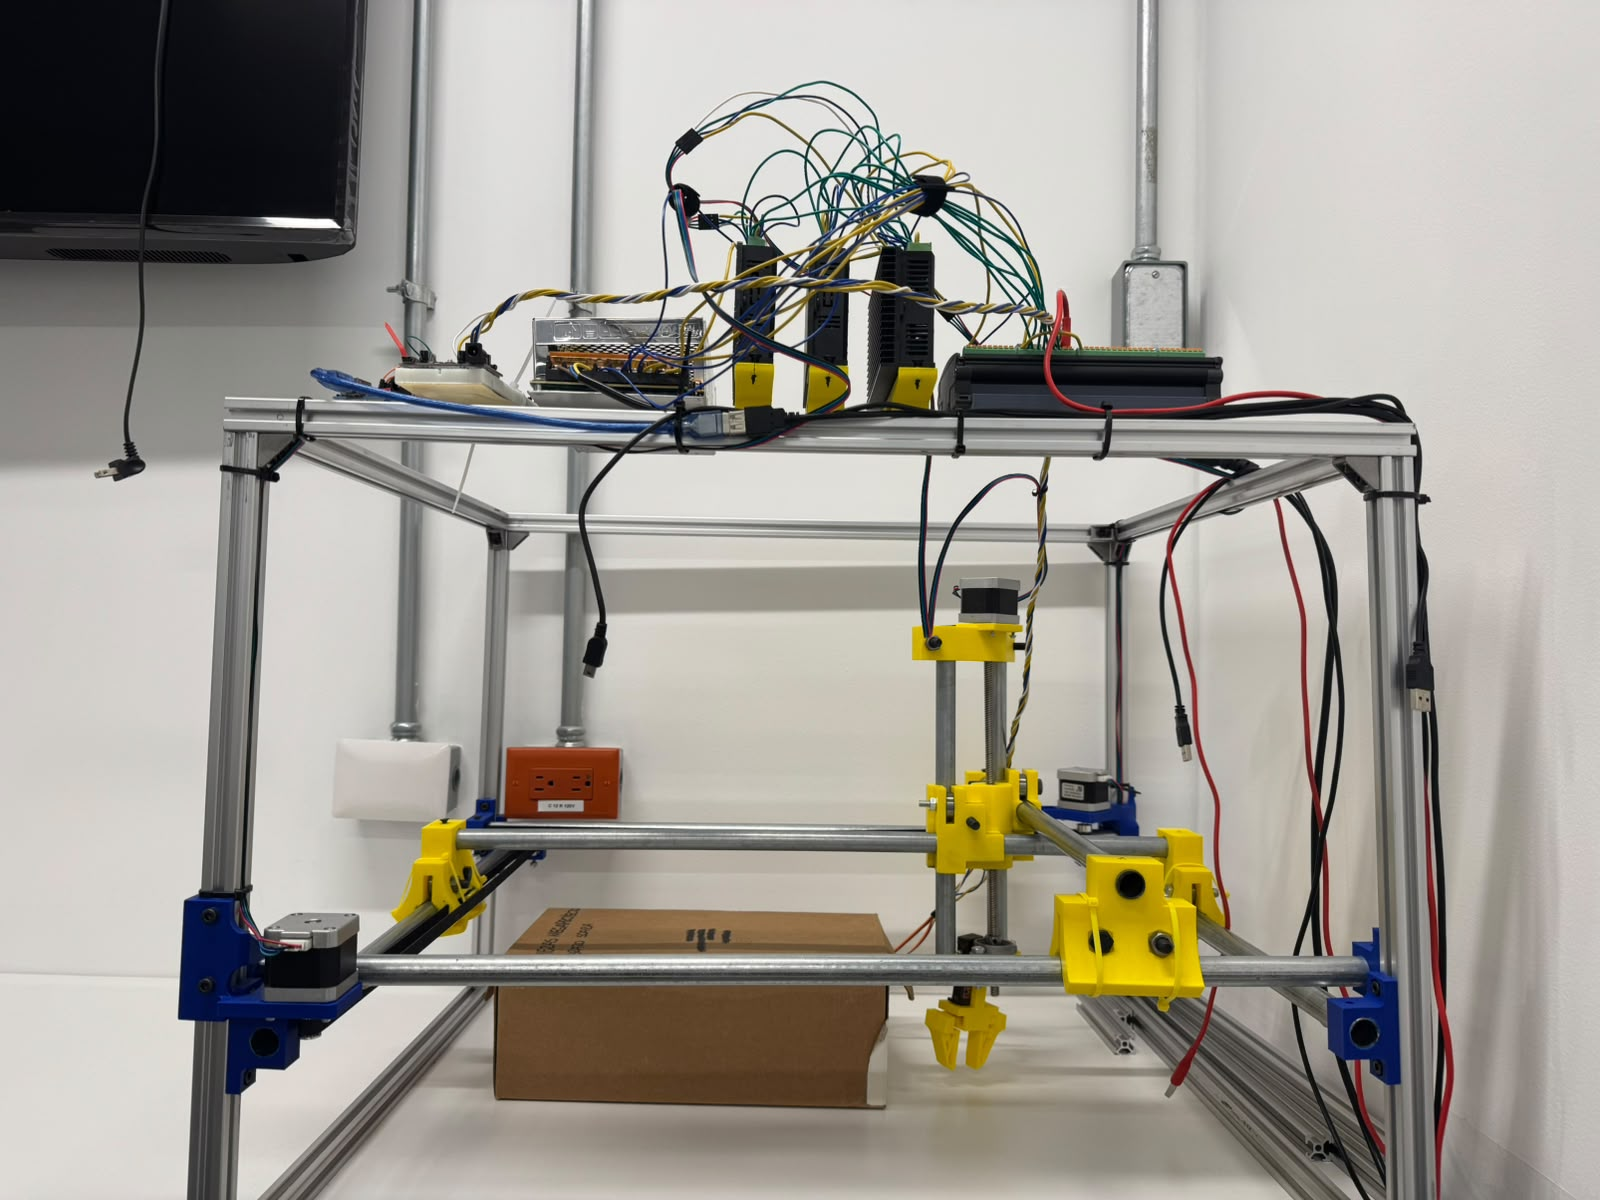
\includegraphics[width=0.75\textwidth,height=6cm,keepaspectratio]{Imagenes de Documentacion/F1_1.jpeg}
    \caption{Configuración inicial del brazo robótico cartesiano.}
    \label{fig:fase1_vista_general}
    \par\small Fuente: elaboración propia.
\end{figure}

En los cuatro carros de X y Y se observó resistencia al desplazamiento y falta de alineación con las guías. También se identificó contacto entre las piezas plásticas y los tubos (Figura~\ref{fig:fase1_carro_xy}). Durante el movimiento del pórtico se observó un avance desigual de sus extremos, identificado como \textit{gantry racking}.

\begin{figure}[H]
    \centering
    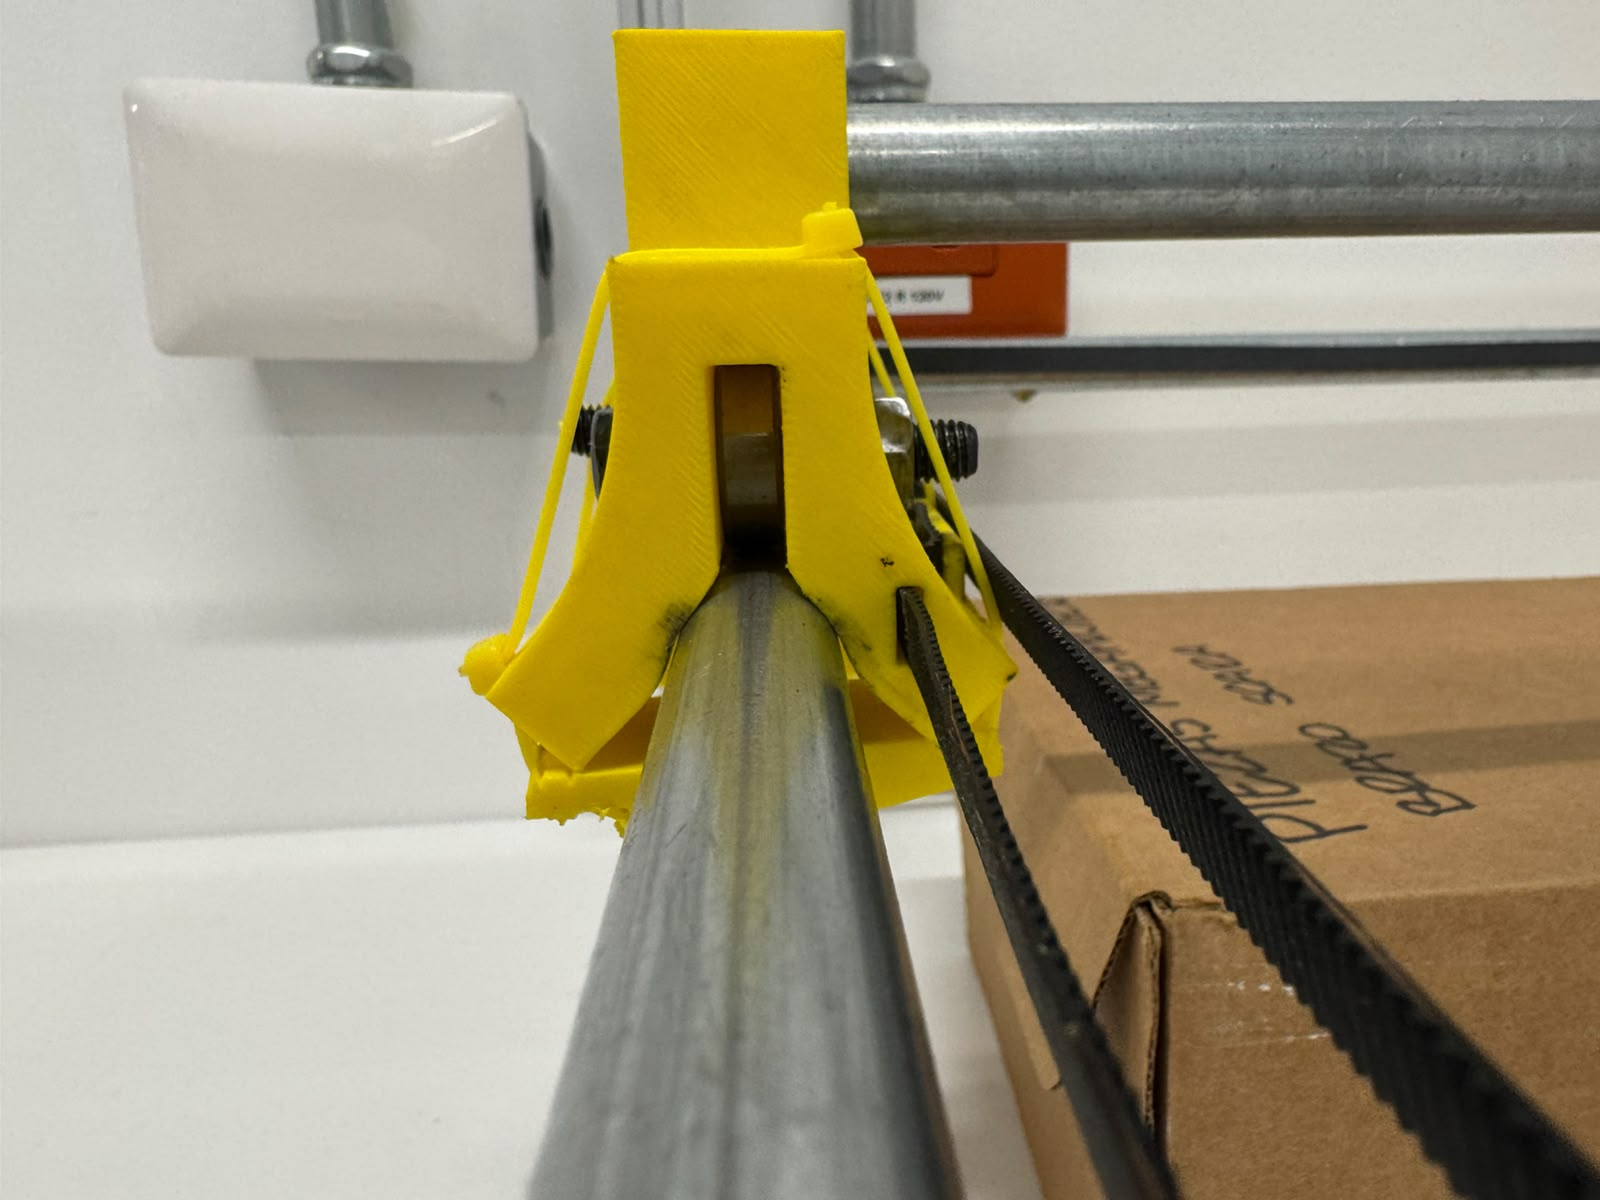
\includegraphics[width=0.65\textwidth,height=5.5cm,keepaspectratio]{Imagenes de Documentacion/F1_3.jpeg}
    \caption{Carro y elementos de guiado del sistema original en X y Y.}
    \label{fig:fase1_carro_xy}
    \par\small Fuente: elaboración propia.
\end{figure}

En Z se observó desalineación del conjunto móvil respecto a la dirección vertical. La disposición del motor, el mecanismo de desplazamiento y la garra se documentó en la Figura~\ref{fig:fase1_eje_z}. Las observaciones de la inspección manual se resumieron en el Cuadro~\ref{tab:fase1_deficiencias}.

\begin{figure}[H]
    \centering
    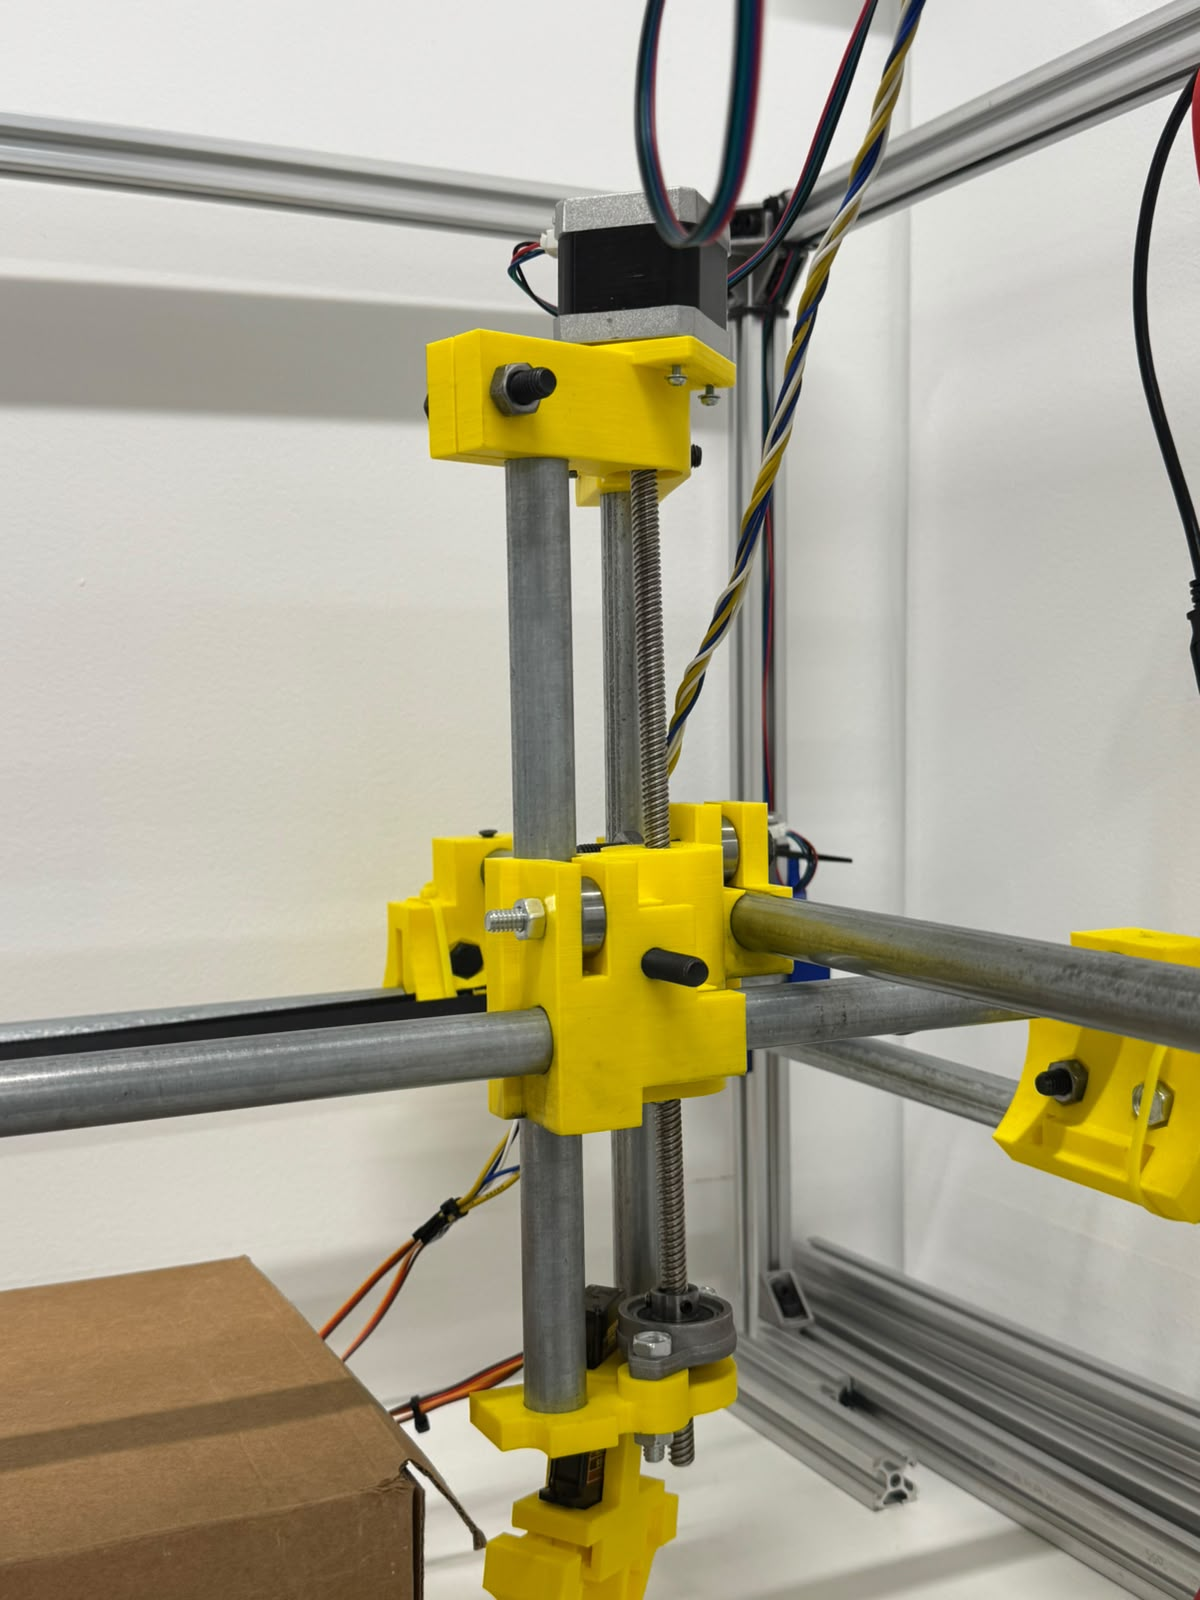
\includegraphics[width=0.55\textwidth,height=5.5cm,keepaspectratio]{Imagenes de Documentacion/F1_4.jpeg}
    \caption{Configuración inicial del mecanismo del eje Z.}
    \label{fig:fase1_eje_z}
    \par\small Fuente: elaboración propia.
\end{figure}

\begin{table}[H]
    \centering
    \caption{Observaciones de la evaluación mecánica inicial.}
    \label{tab:fase1_deficiencias}
    \begin{tabular}{p{0.08\textwidth}p{0.37\textwidth}p{0.43\textwidth}}
        \hline
        Eje & Configuración observada & Hallazgos de la inspección \\
        \hline
        X y Y & Carros impresos con rodamientos radiales sobre tubos metálicos. & Contacto plástico--tubo, resistencia al desplazamiento, desalineación y avance desigual de los extremos del pórtico. \\
        Z & Conjunto vertical con elementos de guiado y soportes impresos. & Desalineación del conjunto móvil y movimiento vertical irregular. \\
        \hline
    \end{tabular}
    \par\small\raggedright Fuente: elaboración propia a partir de la inspección visual y manual.
\end{table}

\section{Fase 2. Selección de componentes y rediseño mecánico}
\label{sec:resultados_fase2}

Se obtuvo un modelo CAD que conservó la arquitectura cartesiana y la disposición general de los ejes X, Y y Z. Se adaptaron los diseños de los soportes de las guías y de los motores de X y Y para incorporar ejes de acero de 12~mm de diámetro. La fabricación de las piezas correspondió a la fase siguiente.

El diseño incluyó cuatro carros para X y Y con rodamientos lineales con carcasa. Cada carro incorporó un paso perpendicular para el eje correspondiente, un espacio para el recorrido de la faja dentada y dos puntos adicionales de fijación (Figura~\ref{fig:fase2_carro_xy}).

\begin{figure}[H]
    \centering
    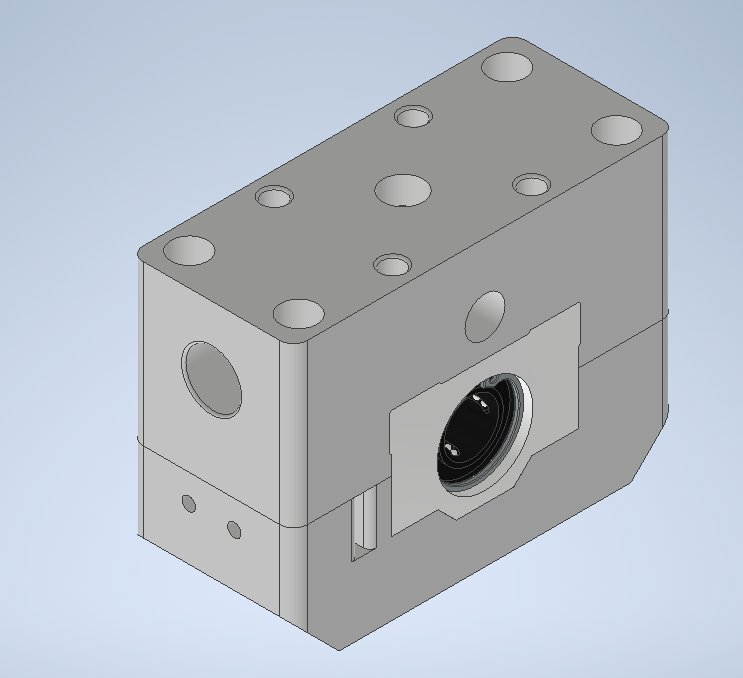
\includegraphics[width=0.65\textwidth,height=5.5cm,keepaspectratio]{Imagenes de Documentacion/F2_1.png}
    \caption{Modelo CAD del carro de traslación de los ejes X y Y.}
    \label{fig:fase2_carro_xy}
    \par\small Fuente: elaboración propia.
\end{figure}

El conjunto central incorporó rodamientos lineales cilíndricos para el desplazamiento en el plano XY. La intersección de ambos ejes quedó ubicada en el centro del conjunto y constituyó la referencia de montaje del mecanismo vertical (Figura~\ref{fig:fase2_centro_xy}).

\begin{figure}[H]
    \centering
    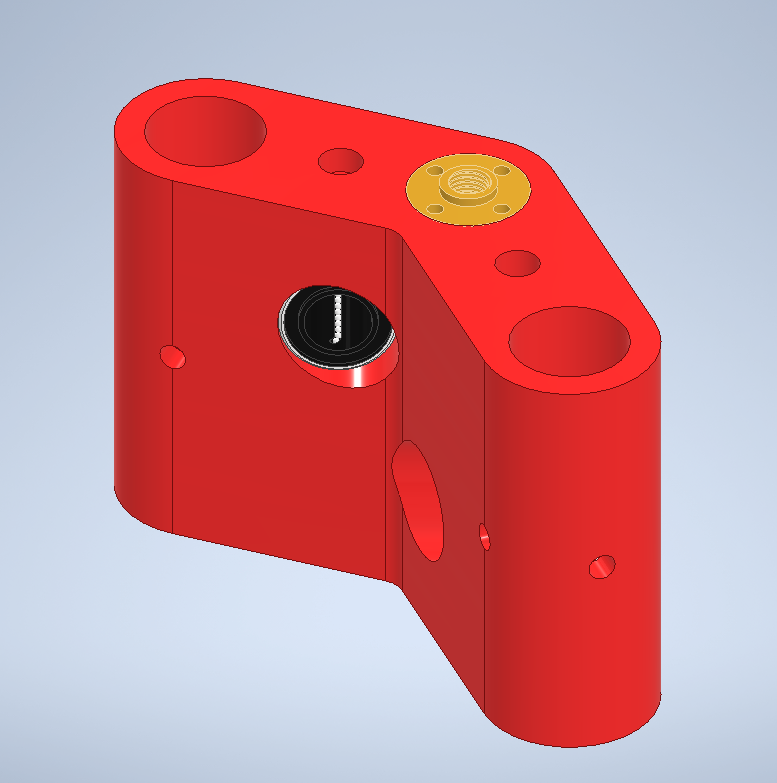
\includegraphics[width=0.65\textwidth,height=5.5cm,keepaspectratio]{Imagenes de Documentacion/F2_2.png}
    \caption{Modelo CAD del conjunto central del mecanismo cartesiano.}
    \label{fig:fase2_centro_xy}
    \par\small Fuente: elaboración propia.
\end{figure}

En el ensamblaje digital, Z incorporó dos guías y un tornillo de avance. Los soportes superior e inferior mantuvieron la separación entre centros definida en el conjunto central (Figura~\ref{fig:fase2_eje_z}). La integración de los componentes se documentó en el ensamblaje general de Autodesk Inventor (Figura~\ref{fig:fase2_ensamble_final}).

\begin{figure}[H]
    \centering
    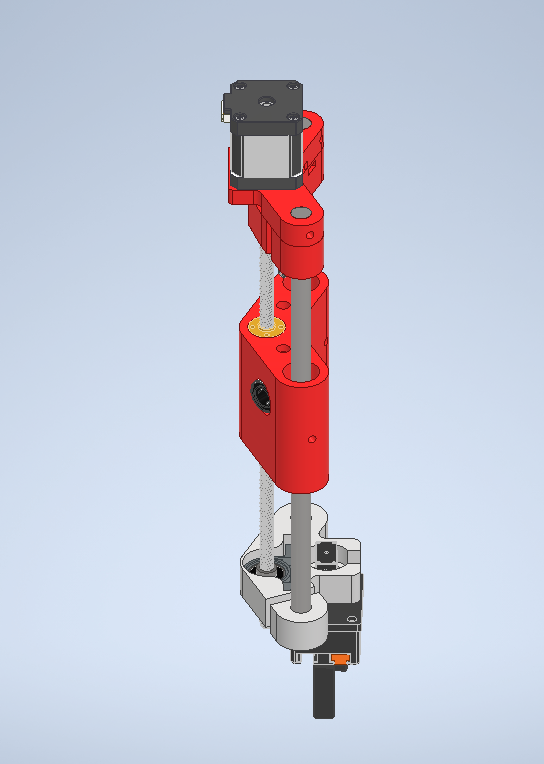
\includegraphics[width=0.60\textwidth,height=6cm,keepaspectratio]{Imagenes de Documentacion/F2_3.png}
    \caption{Modelo CAD del mecanismo vertical integrado al conjunto central.}
    \label{fig:fase2_eje_z}
    \par\small Fuente: elaboración propia.
\end{figure}

\begin{figure}[H]
    \centering
    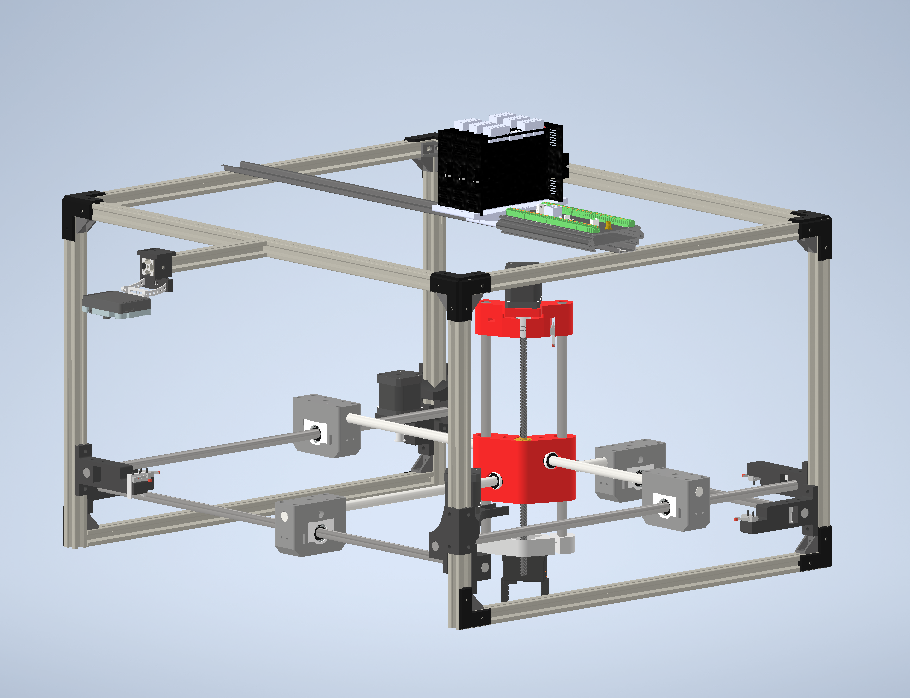
\includegraphics[width=0.75\textwidth,height=6cm,keepaspectratio]{Imagenes de Documentacion/F2_4.png}
    \caption{Ensamblaje CAD del brazo robótico cartesiano en Autodesk Inventor.}
    \label{fig:fase2_ensamble_final}
    \par\small Fuente: elaboración propia.
\end{figure}

% PENDIENTE: confirmar si las imágenes CAD correspondieron a la versión previa
% a fabricar o a una actualización posterior. No se les asignó una iteración.

\section{Fase 3. Implementación mecánica}
\label{sec:resultados_fase3}

\subsection{Componentes fabricados y configuración ensamblada}

Se incorporaron 48 piezas impresas en PLA, incluidas las escuadras de acabado estético. El consumo aproximado de material fue de 1.5~kg, incluidas las pruebas y las iteraciones de fabricación. Todas las piezas impresas se fabricaron nuevamente, incluso aquellas cuyos diseños se retomaron del mecanismo original.

Las piezas obtenidas incluyeron soportes de ejes guía, soportes de montaje de motores, carros de desplazamiento, piezas del conjunto central y soportes de Z. Parte de estos componentes se documentó en la Figura~\ref{fig:fase3_fabricacion}.

\begin{figure}[H]
    \centering
    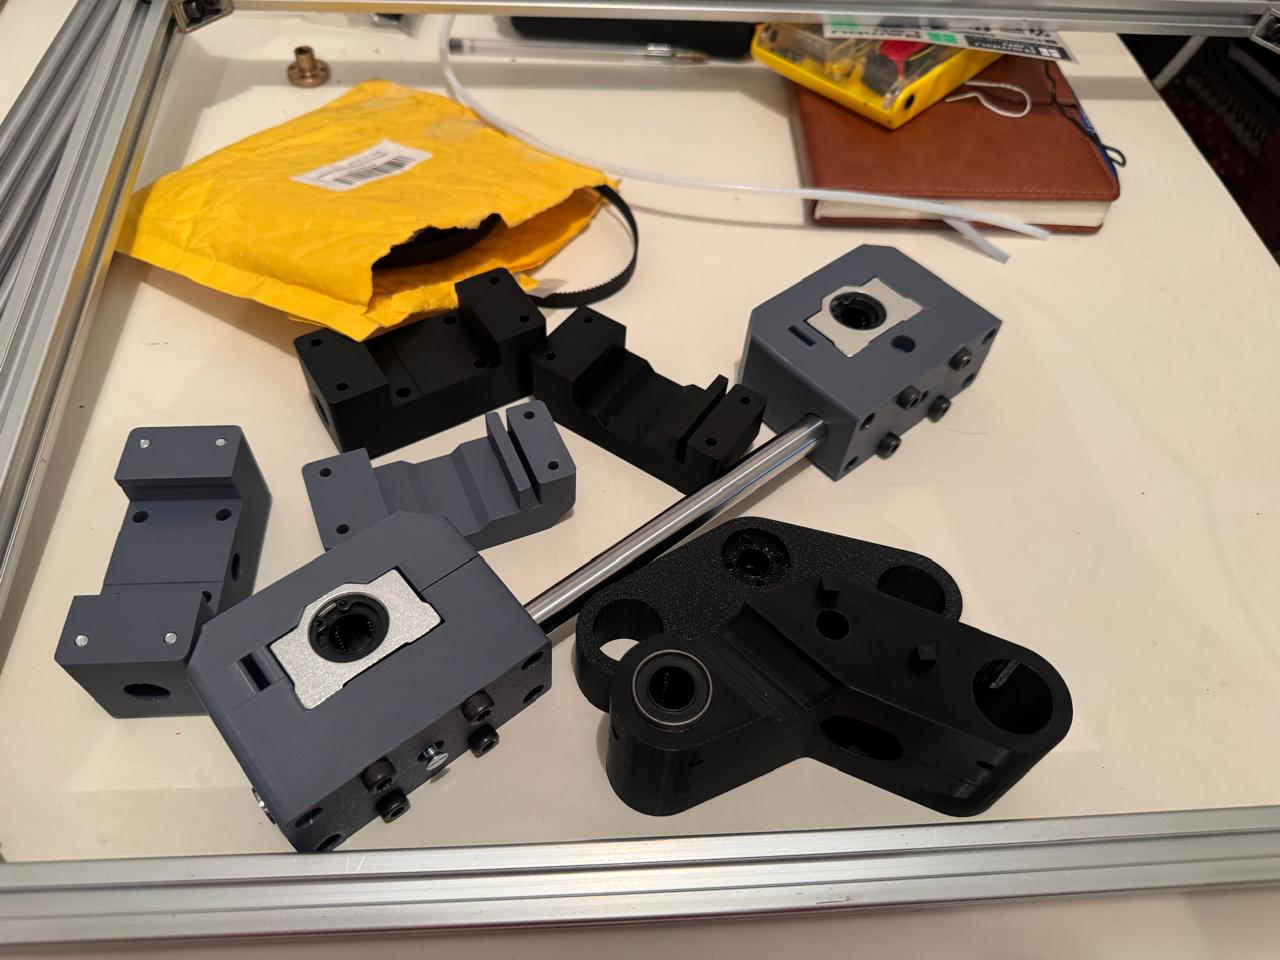
\includegraphics[width=0.72\textwidth,height=6cm,keepaspectratio]{figuras/fase3_componentes.jpeg}
    \caption{Componentes impresos y rodamientos preparados para el ensamblaje.}
    \label{fig:fase3_fabricacion}
    \par\small Fuente: elaboración propia.
\end{figure}

El conjunto ensamblado incorporó perfiles de aluminio 2020 de ranura en T, guías de acero de 12~mm, rodamientos lineales, fajas dentadas para X y Y y un tornillo de avance para Z. Las dimensiones y cantidades reportadas se organizaron en el Cuadro~\ref{tab:fase3_caracteristicas}.

\begin{table}[H]
    \centering
    \caption{Características del conjunto mecánico implementado.}
    \label{tab:fase3_caracteristicas}
    \begin{tabular}{p{0.53\textwidth}p{0.36\textwidth}}
        \hline
        Característica & Valor o configuración \\
        \hline
        Dimensiones generales de la estructura & $700 \times 580 \times 420$~mm \\
        Recorrido reportado del eje X\textsuperscript{a} & 446~mm \\
        Recorrido reportado del eje Y\textsuperscript{a} & 337~mm \\
        Recorrido del eje Z & \textit{Pendiente de medición} \\
        Diámetro de los ejes guía & 12~mm \\
        Ejes de 700~mm & 3 unidades \\
        Ejes de 580~mm & 3 unidades \\
        Perfiles estructurales & Aluminio 2020 de ranura en T \\
        Piezas impresas incorporadas & 48 unidades \\
        Material de las piezas impresas & PLA \\
        Consumo aproximado de PLA, incluidas las pruebas & 1.5~kg \\
        Transmisión en X y Y & Fajas dentadas \\
        Transmisión en Z & Tornillo de avance \\
        \hline
    \end{tabular}
    \par\small\raggedright Fuente: elaboración propia a partir de los datos de fabricación y ensamblaje del proyecto.
    \par\small La altura se refirió a la superficie de la mesa. El consumo de PLA incluyó las pruebas y no correspondió a la masa del brazo ensamblado.
    \par\small\textsuperscript{a} Se conservaron los valores reportados; su procedencia, del modelo CAD o de medición física, quedó pendiente de confirmación.
\end{table}

\subsection{Configuraciones del conjunto central y del soporte de la garra}

El conjunto central pasó por tres iteraciones. En las dos primeras se presentaron dificultades de retención de los rodamientos; en la configuración final estos permanecieron en sus alojamientos durante las comprobaciones de movimiento. Las configuraciones y sus observaciones se resumieron en el Cuadro~\ref{tab:fase3_iteraciones}.

\begin{table}[H]
    \centering
    \caption{Iteraciones del conjunto central y observaciones de montaje.}
    \label{tab:fase3_iteraciones}
    \begin{tabular}{p{0.10\textwidth}p{0.38\textwidth}p{0.40\textwidth}}
        \hline
        Iteración & Configuración & Observación \\
        \hline
        Primera & Cuerpo inicial al que se añadieron tornillos de presión. & Se observó la salida de los rodamientos de sus alojamientos antes de incorporar los tornillos. \\
        Segunda & Conjunto dividido en tres piezas con tornillos de presión. & Persistieron las dificultades de sujeción de los rodamientos. \\
        Tercera & Conjunto con tornillos de unión entre las piezas. & Los rodamientos permanecieron en sus alojamientos durante las comprobaciones realizadas. \\
        \hline
    \end{tabular}
    \par\small\raggedright Fuente: elaboración propia a partir de la descripción del proceso de fabricación y ensamblaje.
\end{table}

El conjunto central ensamblado y una vista del montaje parcial se documentaron en la Figura~\ref{fig:fase3_montaje}. El soporte inferior de Z incorporó una unión desmontable para la garra, en sustitución de la unión fija inicial. El efector final quedó ubicado en la intersección de los ejes del conjunto central.

\begin{figure}[H]
    \centering
    \begin{minipage}[b]{0.38\textwidth}
        \centering
        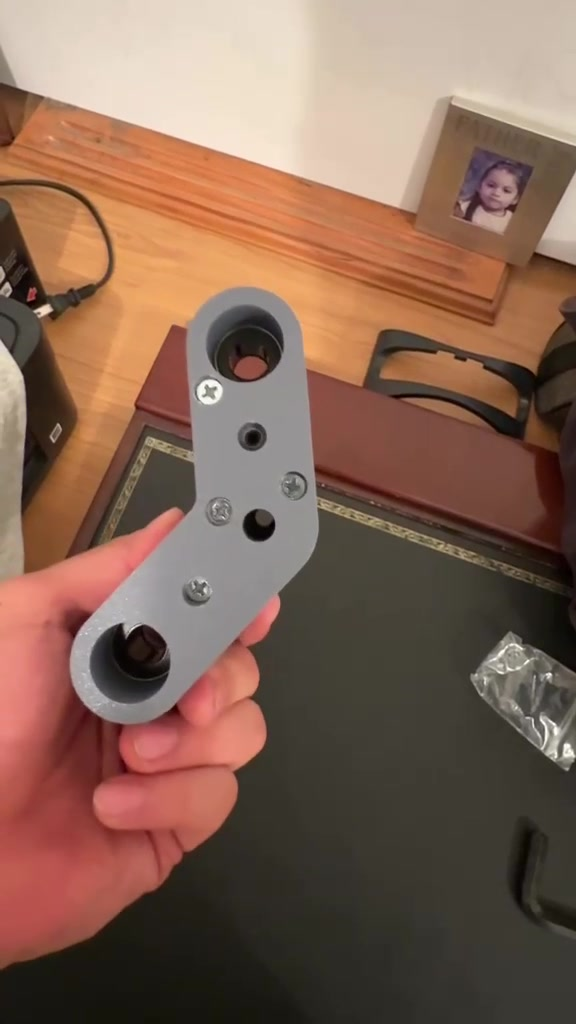
\includegraphics[width=\linewidth,height=6.5cm,keepaspectratio]{figuras/fase3_central_inferior.jpg}
        \par\small (a) Conjunto central ensamblado.
    \end{minipage}
    \hfill
    \begin{minipage}[b]{0.58\textwidth}
        \centering
        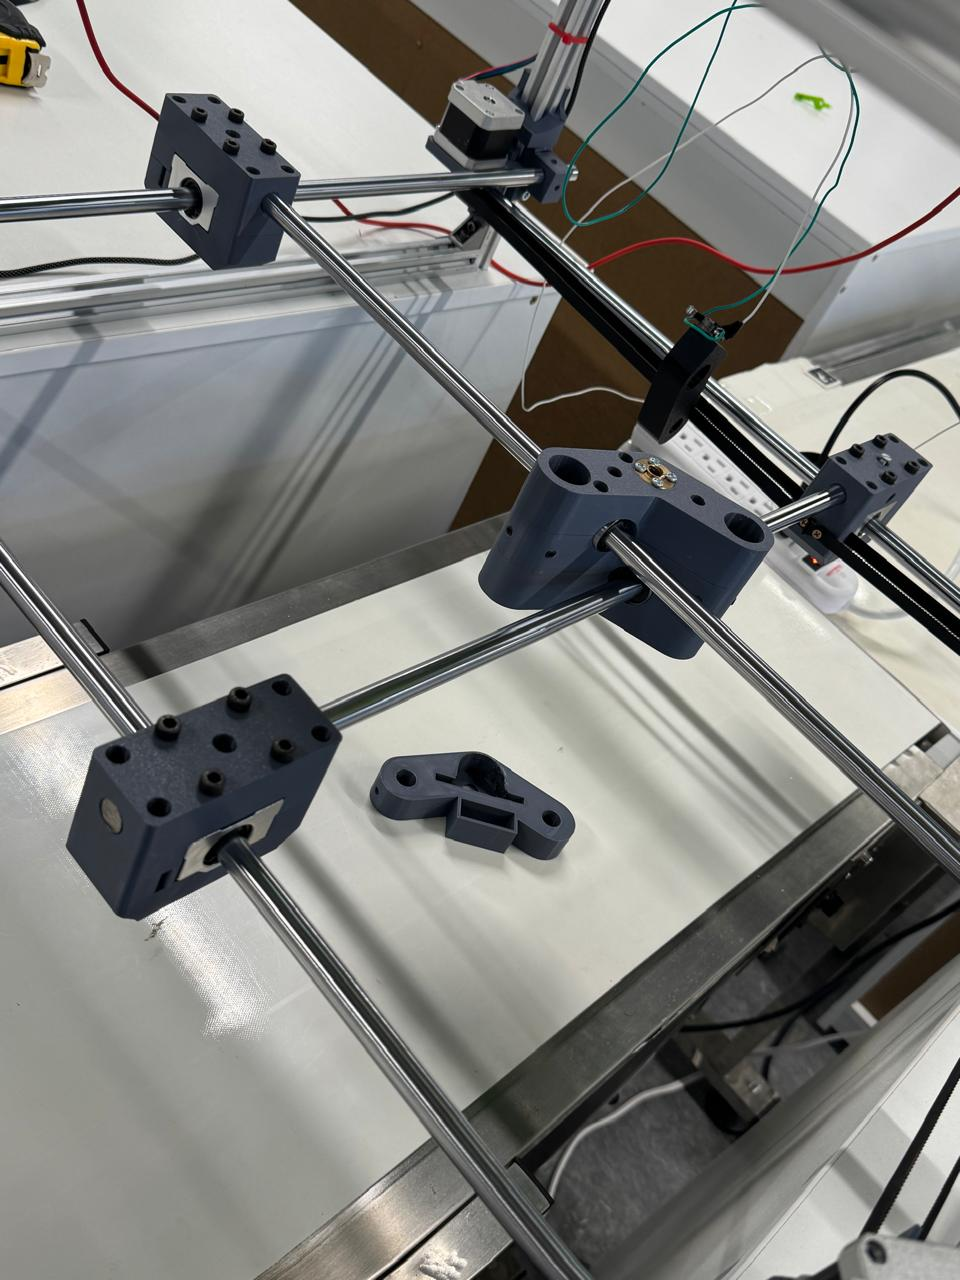
\includegraphics[width=\linewidth,height=6.5cm,keepaspectratio]{figuras/fase3_ensamblaje_parcial.jpeg}
        \par\small (b) Montaje parcial de guías y carros.
    \end{minipage}
    \caption{Conjunto central y montaje parcial del mecanismo cartesiano.}
    \label{fig:fase3_montaje}
    \par\small Fuente: elaboración propia; fotografía y fotograma del registro audiovisual del proyecto.
\end{figure}

\subsection{Comprobación mecánica preliminar}

Se comprobó el desplazamiento de los tres ejes mediante manipulación directa, antes del accionamiento electrónico. Los carros permanecieron sobre sus guías y no se reprodujeron los atascos identificados en el mecanismo original durante las comprobaciones realizadas.

La resistencia al movimiento se percibió menor que en el sistema original. El avance desigual de los extremos del pórtico resultó poco perceptible durante la inspección visual. Se observaron vibraciones leves y no se identificó deflexión de las guías a simple vista. Estas observaciones fueron cualitativas y no correspondieron a mediciones de precisión o repetibilidad.

    \fi  
\fi

% ================================================================================
% DISCUSION
% ================================================================================
\ifdefined\CAPdicusion
	\newpage
	\chapter{Discusión}
	\ifdefined\parpordefecto
    	\defaultparformat{Discusion}
    \else
    	\section{Fase 1. Evaluación del sistema original}

La inspección inicial orientó la intervención hacia los mecanismos de guiado y traslación. El contacto entre las piezas plásticas y los tubos se interpretó como un factor que contribuyó a la resistencia observada durante el movimiento. Esta interpretación se basó en la inspección del conjunto y no en una medición independiente de las fuerzas de fricción.

En X y Y, la desalineación y el avance desigual de los extremos del pórtico se relacionaron con las dificultades de desplazamiento de los carros. El comportamiento de tipo \textit{gantry racking} mostró que el movimiento del conjunto no fue uniforme. No se aisló experimentalmente la contribución de cada componente, por lo que la evaluación identificó condiciones de montaje asociadas con el problema, sin establecer una causa única.

En Z, la desalineación del motor, el mecanismo de desplazamiento y la garra indicó la necesidad de revisar la geometría del conjunto vertical. El rediseño se orientó a establecer una disposición común de sus guías y soportes, en lugar de limitar la intervención al contacto entre los carros y las guías.

Estos hallazgos aportaron el diagnóstico mecánico correspondiente al primer objetivo específico. La selección de componentes y el rediseño se desarrollaron en la segunda fase; la fabricación y la comprobación del mecanismo modificado correspondieron a la tercera. La inspección inicial no permitió cuantificar la precisión ni la repetibilidad del sistema original.

\section{Fase 2. Selección de componentes y rediseño mecánico}

La conservación de la arquitectura cartesiana respondió a que las deficiencias identificadas se concentraron en el guiado y la traslación. Por ello, se retomaron los diseños de los soportes de los ejes y de los motores de X y Y y se adaptaron a guías de acero de 12~mm. Esta decisión conservó parte de la geometría aprovechable del sistema, sin reutilizar las piezas impresas originales.

La selección de rodamientos lineales con carcasa facilitó la definición de uniones atornilladas entre los rodamientos y los carros. El modelado a partir de sus dimensiones estableció los espacios de montaje, el paso del eje perpendicular y el recorrido de la faja. En esta fase, el resultado correspondió a una configuración geométrica; su funcionamiento físico se comprobó después de la fabricación.

El conjunto central requirió un diseño específico porque articuló los desplazamientos en X y Y con el montaje del mecanismo vertical. La disposición de los rodamientos definió la separación entre guías y proporcionó una referencia común para los soportes de Z. La ubicación del efector final en la intersección de los ejes respondió a esa organización geométrica, sin constituir por sí sola una validación del posicionamiento del brazo.

Se conservaron las fajas dentadas porque estuvieron disponibles en el laboratorio. En Z se mantuvo el principio de transmisión mediante tornillo de avance y se modificaron los elementos de soporte para atender la desalineación observada. La intervención se concentró, por tanto, en integrar los componentes disponibles con el nuevo sistema de guiado.

La segunda fase aportó el diseño de los sistemas de traslación previsto en el primer objetivo específico. El ensamblaje CAD estableció la disposición de los componentes, pero no sustituyó la comprobación de las tolerancias de fabricación, la retención de los rodamientos ni el comportamiento del mecanismo ensamblado.

\section{Fase 3. Implementación mecánica}
\label{sec:discusion_fase3}

La fabricación y el ensamblaje evidenciaron diferencias entre la definición geométrica del modelo y las condiciones del montaje físico. Las dificultades se concentraron en la retención de los rodamientos del conjunto central, la alineación de las guías y el tensado de las fajas. Su resolución requirió iteraciones sobre los componentes y ajustes durante el montaje.

El PLA se utilizó por tratarse de un material común para impresión tridimensional. La impresión permitió fabricar nuevamente los componentes y modificar sus geometrías durante el desarrollo. Las tolerancias variaron entre piezas, y se identificó la posible necesidad de lijado en superficies curvas para mejorar el acoplamiento. Esta limitación mostró la importancia de comprobar físicamente los ajustes; no se documentó un valor único de tolerancia aplicable al conjunto.

Las tres iteraciones del conjunto central mostraron que facilitar la impresión no resolvió automáticamente la retención de los rodamientos. La división en tres piezas atendió la dificultad de fabricación, pero la disposición de los tornillos de presión se interpretó como una fuente de acciones opuestas que dificultaron la sujeción. La unión atornillada entre las secciones mantuvo los rodamientos en sus alojamientos durante las comprobaciones realizadas. El resultado vinculó la facilidad de fabricación con la necesidad de definir cómo quedaron unidas las piezas.

La alineación de las guías también condicionó el ensamblaje. El traslado de las distancias del modelo de Inventor al montaje proporcionó referencias para posicionar los soportes y facilitó esta operación. La ausencia de atascos en las comprobaciones posteriores fue compatible con una mejora del guiado, aunque no permitió separar el efecto de los nuevos rodamientos del efecto de los ajustes de alineación.

La fijación de las fajas mediante tornillos resolvió el montaje y el tensado necesarios para las comprobaciones iniciales. Sin embargo, no se midió la tensión ni se evaluó la durabilidad de las zonas perforadas. Del mismo modo, las arandelas se incorporaron con la intención de reducir el riesgo de aflojamiento, sin una evaluación específica de la conservación del apriete durante el uso prolongado. El alcance de estas soluciones quedó limitado a las condiciones comprobadas durante el montaje.

El soporte inferior desmontable de Z atendió la necesidad de retirar la garra para almacenar el equipo. El aporte del proyecto correspondió a su soporte y a la integración con el mecanismo vertical; la geometría original de la garra procedió de un modelo externo.\footnote{La identificación del autor y de la fuente del modelo de la garra quedó pendiente de documentación.}

La menor resistencia percibida, la ausencia de atascos durante las comprobaciones y la reducción visual del avance desigual del pórtico respaldaron una mejora cualitativa del movimiento. No se cuantificaron la fricción, la deflexión ni el desfase entre los extremos, por lo que estas observaciones no demostraron su eliminación completa ni una mejora medida de precisión o repetibilidad.

La tercera fase aportó la materialización y la comprobación mecánica preliminar del rediseño asociado con el primer objetivo específico. El desplazamiento a mano de los tres ejes estableció una base para las pruebas posteriores de accionamiento electrónico. Esta comprobación se distinguió del modo manual mediante mando inalámbrico y no sustituyó la validación experimental prevista en las fases posteriores.

    \fi  
\fi

% ================================================================================
% Conclusiones
% ================================================================================
% \ifdefined\CAPconclusiones
% 	\newpage
% 	\chapter{Conclusiones}
% 	\ifdefined\parpordefecto
% 		\defaultparformat{conclusiones}
% 	\else
% 		\input{conclusiones}
% 	\fi
% \fi

% ================================================================================
% RECOMENDACIONES
% ================================================================================
% \ifdefined\CAPrecomendaciones
% 	\newpage
% 	\chapter{Recomendaciones}
% 	\ifdefined\parpordefecto
% 		\defaultparformat{recomendaciones}
% 	\else
% 		\input{recomendaciones}
% 	\fi
% \fi

% ================================================================================
% CAPÍTULOS
% ================================================================================
% \newpage
% \ifdefined\parpordefecto
% 	\defaultparformat{capitulos}
% \else
% 	\chapter{Derivación de la dinámica del mecanismo}

\section{Dinámica de cuerpos rígidos}

\section{Restricciones}
\subsection{Mecanismos de lazo cerrado}
\subsubsection{Mecanismo de cuatro barras}

\chapter{Control del sistema mecánico}

\section{La ecuación del manipulador}
% \fi





% BIBLIOGRAFÍA
% % --------------------------------------------------------------------------------
\ifdefined\CAPbibliografia
	\newpage
	\cleardoublepage\phantomsection
	\addcontentsline{toc}{chapter}{Bibliografía}
	\ifdefined\usarAPA
		\bibliographystyle{apacite}
	\else
		\bibliographystyle{babplain}
	\fi
	\nocite{*}
	\bibliography{bibliografia}
\fi

% % ANEXOS
% % --------------------------------------------------------------------------------
% \ifdefined\CAPanexos
% 	\newpage
%     \cleardoublepage\phantomsection
%     \begin{center}
%     	\vspace*{\fill}
%     	\Huge Anexos
%     	\vspace*{\fill}
%     \end{center}
%     \addcontentsline{toc}{chapter}{Anexos}
%     \renewcommand{\chaptername}{Anexo}
%    \setcounter{chapter}{0}
% 	\renewcommand{\thechapter}{\Alph{chapter}}
% 	\ifdefined\parpordefecto
%     	\defaultparformat{anexos}
%     \else
%     	\chapter{Planos de Construcción}
%     \fi
% \fi

% GLOSARIO
% % --------------------------------------------------------------------------------
\ifdefined\CAPglosario
	\newpage
	\printglossary
\fi

% % LISTADO DE SÍMBOLOS
% % --------------------------------------------------------------------------------
% \ifdefined\CAPsimbolos
% 	\newpage
%     \cleardoublepage\phantomsection
%     \printnomenclature
% \fi

\end{document}
